
\section{Introduction}
\label{chp:understanding_understandability}

Search engines are concerned with retrieving relevant information to support a user's information seeking task. Commonly, signals about the topicality or aboutness of a piece of information to a query are used to estimate relevance, with other relevance dimensions like understandability, trustworthiness, etc.~\cite{} being relegated to a secondary position, or completely neglected. While this may be a minor problem for many information seeking tasks, there are some specific tasks in which dimensions other than topicality have an important role in the information seeking and decision making process. The seeking of health information and advice on the Web by the general public is one such task. 

A key problem when searching the Web for health information is that this can be too technical, unclear, unreliable, generally misleading, and can lead to unfounded escalations and poor decisions~\cite{white09b}. Where correct information exists, it can be hard to find amongst the noise, spam, and irrelevant information. In \textit{high-stakes search tasks} such as this, access to poor information can lead to poor decisions which ultimately can have a significant impact on our health and well-being~\cite{white09b,white13}. In this work we are specifically interested in the understandability of health information retrieved by search engines, and in improving search results to favour information understandable by the general public. 

The use of general purpose Web search engines like Google and Bing for seeking health advice has been largely questioned and criticised~\cite{graber99readability,fitzsimmons2010readability,wiener2013readability,patel13readability,atcherson14readability,meillier17readability}, despite the commendable efforts these players have put in providing increasingly better health information to their users, e.g., the Google Health Cards~\cite{}. 

Ad-hoc solutions to support the general public in searching and accessing health information on the Web have been implemented, typically supported by governments initiatives or medical practitioners associations, e.g., HealthDirect.gov.au, HealthOnTheNet.org. These solutions aim to provide \textit{better} health information to the general public. For example, Health On The Net's mission statement is ``to guide Internet users to reliable understandable accessible and trustworthy sources of medical and health information''. But, do the solutions these services currently employ actually provide this type of information to the health-seeking general public? As an illustrative example, we analysed the top 10 search results retrieved by Health On The Net and Health Direct\footnote{Results retrieved on XXX.} in answers to 300 search queries used within the CLEF 2016 Ehealth evaluation task (see Section~\ref{}). Table/Figure~\ref{} reports the distribution of understandability scores for these search results (note, we did not assess the topical relevance of these results). Understandability scores were computed with the most effective estimation methods from Section~\ref{}. For comparison, we report also the distribution of understandability scores of the ``optimal'' search results for those queries, as found from the CLEF 2016 Ehealth evaluation task (relevant results that have the highest understandability scores). The results clearly indicate that, despite these solutions are expressively aimed at supporting the general public in accessing understandable health information, they often fail to do so.

In this paper we propose and investigate methods for the estimation of understandability for health information in Web pages. In doing so, we also study the influence of HTML processing methods on these estimations, and their pitfalls. Then, we investigate how understandability estimations can be integrated into retrieval methods to enhance the quality of the retrieved health information, with particular attention to its understandability by the general public. 

%==== ARRIVED TO HERE =====
%
%
%An existing concern of communicators is knowing if their message is well understood by their target public.  
%Writing for a group of readers other than one's own is difficult.
%This fact motived research over the past century on the development of readability formulas which can, through a single number, provide hints on the difficulty of a text.
%Readability formulas were then widely adopted by different groups of the society, showing their effectiveness when increasing the amount learnt by recruits in the army \cite{klare55} or the readership of newspaper \cite{perry54}.
%%became popular and are widely used. For example, different news outlets have are targeting different audiences: TV Guide....NewYorkTimes....
%%....being implemented, for instance, in the Microsoft office package\footnote{\url{https://support.office.com/en-us/article/Test-your-document-s-readability-85b4969e-e80a-4777-8dd3-f7fc3c8b3fd2#ID0EAADAAA=2016,_2013,_2010}}.
%
%Nevertheless, with advent and popularity of Web, in which anyone can write about anything, content has been largely generated without proper concern with its understandability.
%Again: writing for a group of readers other than one's own is difficult and in some domains this might be dangerous.
%The medical domain is one of such \cite{}.
%The problem, as reported by X, is that health consumers might put themselves at risk if they misunderstand the content of what they read on the Web \cite{}.
%Typically health consumers, such as patients and their next-of-kin, start their searches through commercial search engines \cite{}.
%Thus, researchers in various areas of medicine have assessed the understandability of the material retrieved by popular search engines, often finding that they are harder to understand than they should be (e.g., \cite{graber99readability,fitzsimmons2010readability,wiener2013readability,patel13readability,atcherson14readability,meillier17readability}).
%Mostly, this kind of research also relies on the output of readability formulas to deem if a Web page is easy or hard to understand.
%
%However, as recently discussed in Palotti et al.\cite{palotti15}, the automated use of readability formulas firstly requires the content extraction from Web documents.
%Palotti identified that the decision of appending a period at the end of each element in a list or table extracted from the HTML might result either in a single very long or many very short sentences, 
%which drastically affects the interpretation of readability formula results. The same readability formula may yield results that vary from \textit{suitable even for kids} to \textit{understandable only if you are an experts} with only adding or removing a single period, a 'minor' implementation decision when cleaning HTML pages. 
%One limitation of Palotti's work is not evaluating if either of these interpretations is correct.
%
%In this paper, we propose a vast investigation on the preprocessing of Web documents and the correlation of their understandability estimation with human assessments.
%For that, we take advantage of the understandability assessments made in recent Information Retrieval campaigns in CLEF eHealth (\cite{clef15,clef16}).
%
%%\todo{Should we detail the tasks?} 
%During the CLEF eHealth 2015 and 2016 campaigns \cite{clef15,clef16}, organizers explored Internet communities, such as Reddit AskDocs\footnote{\url{https://www.reddit.com/r/AskDocs/}} - in which people seek medical advice free of charge, to generate health consumer searches. Participants in CLEF eHealth campaigns were then instruct to search a considerable portion of the Web\footnote{In 2016 campaing ClueWeb-12 B was used: \url{http://lemurproject.org/clueweb12/}} for documents that could be topically relevant for each consumer query.
%In addition to topical relevance, medical students and health professionals serving as assessors were instructed to assess how easy to understand and how much they would trust the information contained in each assessed document. % The assessment tool used in these campaigns is shown in Figure~\ref{fig:relevation} to enhance the reader understanding.
%%
%In this work, we extensively use the understandability assessments collected in these campaigns.
%%We limit our analysis to the relevant documents to reduce the noise associated with understandability assessments, as the use of ClueWeb-12 B in 2016 campaign resulted in documents from a broad range of topics being retrieved, not only medical ones, and we would like to keep in our analysis only documents related to medicine.
%
%%As also depicted in Figure~\ref{fig:relevation}, understandability assessments were given on a 4-label scale (scores from 0 to 3) in 2015 and on a 0-100 scale in 2016.
%%Easy to understand documents had assessments closer to 0 while hard to understand document had their assessments close to the maximal value, 3 in 2015 and 100 in 2016.
%%Altogether there are 1,452 documents assessed for understandability for CLEF eHealth 2015 and 3,320 for 2016 (see a detailed analysis in Appendix~\ref{apx:clef}, for example, Figures~\ref{fig:boxplot_labels} and~\ref{fig:boxplot_others} report the assessment distribution).
%
%We correlate the human assessments with the output of various readability formulas applied with different preprocessing settings.
%Our first intent is to complete Palotti's work, providing guidelines for the automatic use of these formulas in the Web documents in the medical domain.
%We take advantage of the framework built to further investigate other understandability estimators besides the readability formulas.
%Finally, we use the lessons learnt in our correlation analysis to demonstrate how is possible to retrieve more understandable medical content. 
%
%\todo{add roadmap?}
%
%%We start our experiments in this chapter analysing the correlation of each readability formula to the human assessments, our ground truth, in Section~\ref{sec:which_readability}.
%%We then study other understandability estimators going far beyond the readability formulas. Those are presented in Section~\ref{sec:proxies}.
%%Similarly, to our experiments with readability formulas, we empirically investigate in Section~\ref{sec:beyond_readability} the patterns that lead to effective understandability estimators.
%%In Section~\ref{sec:which_preprocessing} we compare the effect of different preprocessing methods in the light of more than 100 understandability estimators.
%%Our findings and highlights are summarized in Section~\ref{sec:conclusion_doc_analysis}.

\section{Related Work}
\label{sec:related}
There is a large body of literature that has examined the understandability of Web health content when the information seeker is a member of the general public. For example ...
A common finding of these studies is that, in general health content available on Web pages are often hard to understand by the general public; this includes content that is retrieved in top rank positions by current commercial search engines.

Previous Linguistics and Information Retrieval research has attempted to devise computational methods for the automatic estimation of text readability and understandability~\footnote{TODO: difference between readability and understandability}, and for the inclusion of these within search methods. Computational approaches to understandability estimations include (1) readability formulas, which exploit word surface characteristics of the text, (2) matching with specialised dictionaries or terminologies, often compiled with information about understandability difficulty, (3) machine learning approaches.

Measures such as  Coleman-Liau Index (CLI), Dale-Chall Index, XXX (FRE), XXX (SMOG)~\cite{} belong to the first category. These measures generally rely on ...
While these measures have been widely used in studies investigating the understandability of health content retrieved by search engines, e.g.~\cite{becker2004study}, Palotti et al. found that these measures are heavily affected by the methods used to extract text from the HTML source~\cite{palotti15}. They were able to identify specific settings of a HTML preprocessing pipeline that provided consistent  estimates. We shall revisit this work in more details in Section~\ref{sec:which_readability}, as we further investigate this problem by comparing the effect of HTML preprocessing on text understandability estimations in light of explicit human assessments. 


The use of the Consumer Health Vocabulary (CHV) or of terminologies like the MEdical Subject Headings (MESH) belong to the second category. TODO: here speak about CHV, but also about Dawei Song's use of UMLS/Mesh ontology level.

Use of Machine Learning for understandability: anything in health specifically?

%Readability formulas? CLEF work? CIKM paper? White/MSR papers?....???

\section{Which Readability Formula To Use}
\label{sec:which_readability}

%The aim of this section is to study the individual correlation of each traditional readability metric listed in Table~\ref{tab:doc_features}.
%Our goal is to provide guidelines for the use of readability metrics on health Web documents, as typically has been done in various recent works 
%(e.g., \cite{graber99readability,fitzsimmons2010readability,wiener2013readability,patel13readability,atcherson14readability,meillier17readability}) \todo{elaborate on this motivation}. 
%We plotted Figures~\ref{fig:bar_corr_clef15} and~\ref{fig:bar_corr_clef16} focusing on the correlation score of each traditional readability metric of Figures~\ref{fig:boxplot_corr_docs_2015} and~\ref{fig:boxplot_corr_docs_2016}.
% TODO: write about the preprocessing methods here...

Palotti, Zuccon and Hanbury~\cite{palotti15} compared six different HTML cleaning methods and their impact in the use of readability formulas.
They evaluate three methods to extract the content of a Web page from its HTML source: BeautifulSoap 4, which just naively removed HTML tags, Boilerpipe\footnote{Add ref.} and Justext\footnote{Add ref.}, two approaches to eliminate boilerplate text together with HTML tags. Henceforth these methods are referred as \textit{Naive}, \textit{Boilerpipe - Boi} and \textit{Justext - Jst}, respectively.
The authors noticed that the text in HTML tags often missed a correct punctuation mark. For example, the text extract from titles, menus, tables or lists could be interpreted as many short sentences of few very long sentences, depending only whether a period is forced at the end of sentences. These two preprocessing options are henceforth called \textit{ForcePeriod - FP} and \textit{DoNotForcePeriod - DNFP}.

Their experiments found that the use of \textit{Naive} preprocessing was associated with larger variances in the understandability score estimated by readability formulas, while the use of both \textit{Boi} and \textit{Jst} were more stable. Coleman-Liau Index (CLI) was the most stable metric among all tested in Palotti's work\cite{palotti15}.

In our experiments, we use the Pearson, Kendall Tau and Spearman's Rank correlation to compare the understandability label assigned to each document by human assessors and by readability formulas.
Pearson correlation is used to calculate the strength of two linearly related variables, while the Kendall and Spearman are rank correlation, i.e., they act on the rank of the variables instead of their values. We opt to report on all three correlation coefficients as all three are equally used in the literature, and thus we allow other researchers to compare our results across.

We show in Figures~\ref{fig:bar_corr_clef15} and~\ref{fig:bar_corr_clef16} the correlation scores of each traditional readability metric with the human assessments made in CLEF 2015 and 2016, respectively. We observe that the \textit{Naive} preprocessing also results in the lowest
correlation, no matter which correlation measure or readability formula is used. Also, when the \textit{Naive} preprocessing is used, the variant \textit{DoNotForcePeriod} yields higher correlations than the variant \textit{ForcePeriod}, but when using a higher quality HTML cleaner, such as Justext or Boilerplate, the results indicate that the use of \textit{ForcePeriod} should be preferred.

Among all the readability formulas and preprocessing methods, SMOG with \textit{ForcePeriod} preprocessing and Dale-Chall Index with \textit{DoNotForcePeriod} are the best ones respectively for 2015 and 2016. Although there is no single best readability measure or best preprocessing strategy in all scenarios, CLI and FRE with \textit{Justext} are stable options, with correlation coefficients as high as the best ones in both campaigns. Thus, we confirm Palotti's advice for the use of CLI, as it
has shown once more to be the most robust measure to variances due to use of \textit{ForcePeriod} or \textit{DoNotForcePerid}.


\begin{figure}[th!]
   \centering
   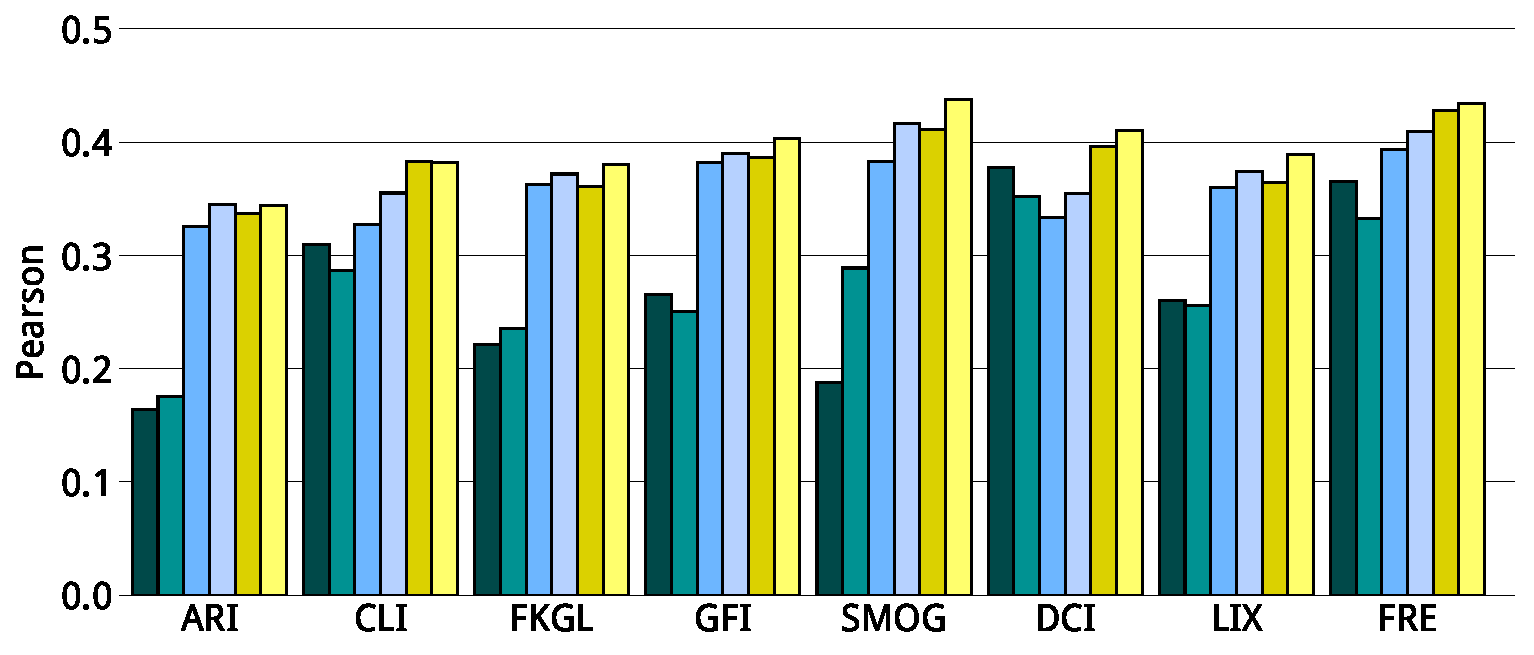
\includegraphics[width=1.\textwidth]{graphics/bar_corr_pearson15_values}
   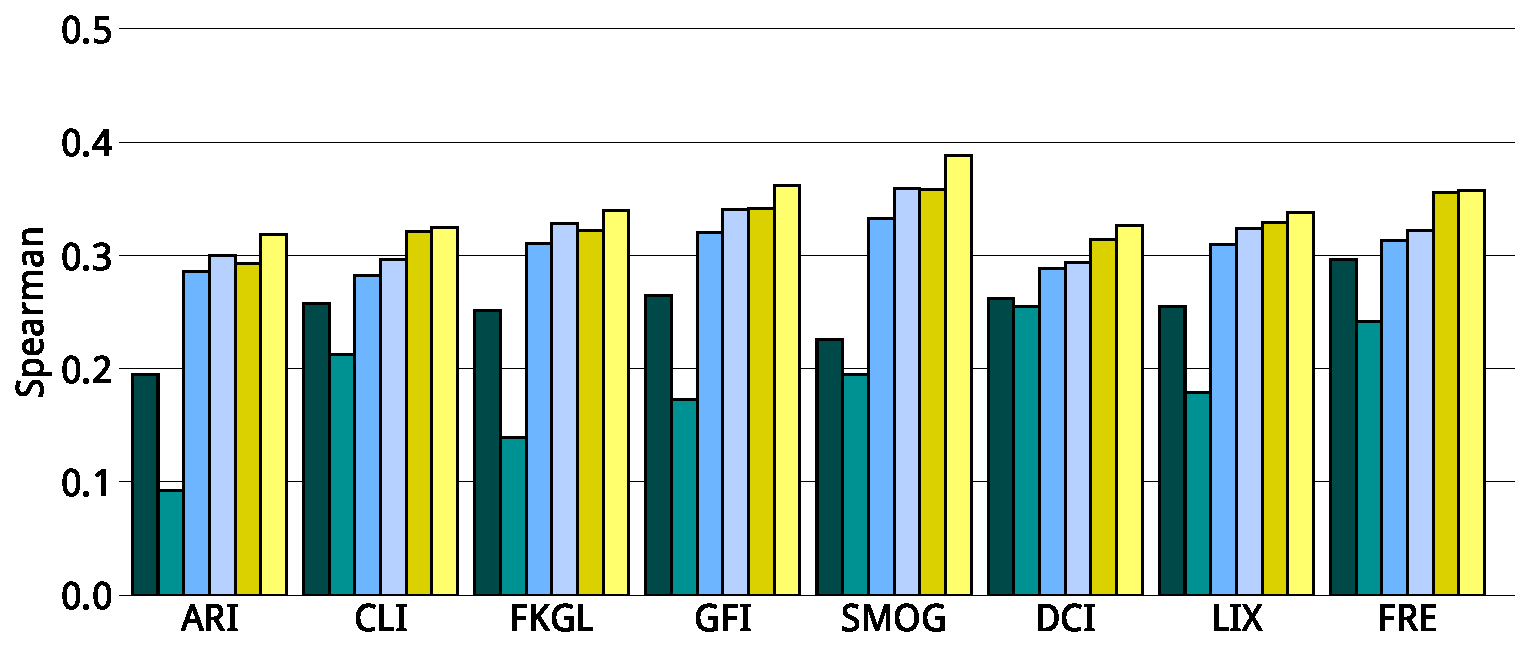
\includegraphics[width=1.00\textwidth]{graphics/bar_corr_spearman15_values}
   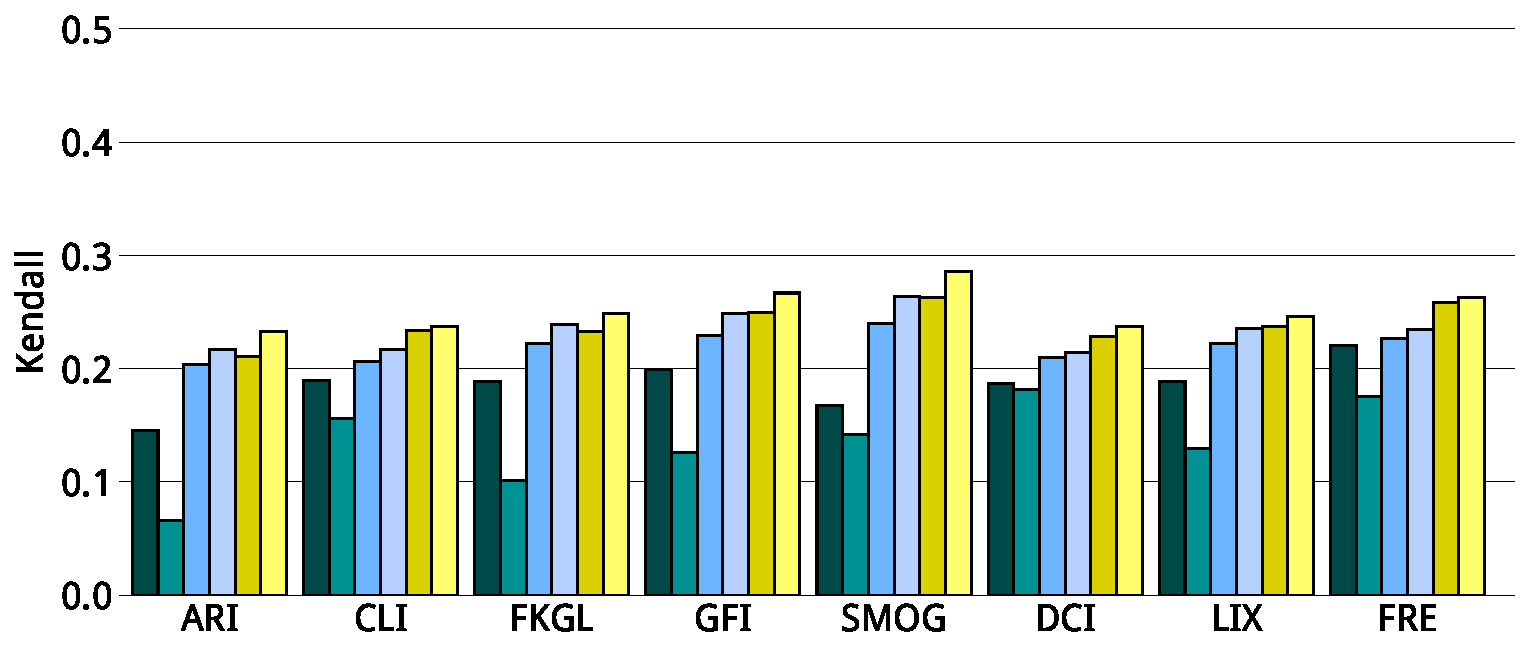
\includegraphics[width=1.00\textwidth]{graphics/bar_corr_kendalltau15_values}
   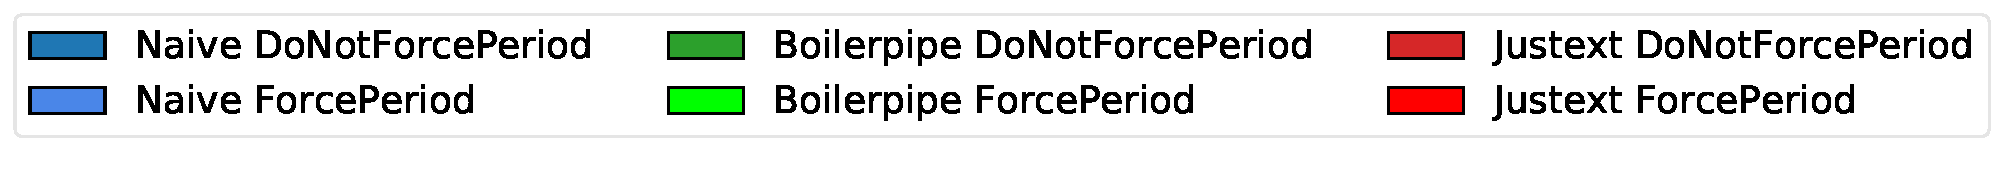
\includegraphics[width=1\textwidth]{graphics/legend62}
    \caption{Correlation of different readability measures and the understandability scores collected in CLEF eHealth 2015}
   \label{fig:bar_corr_clef15}
\end{figure}

\begin{figure}[th!]
   \centering
    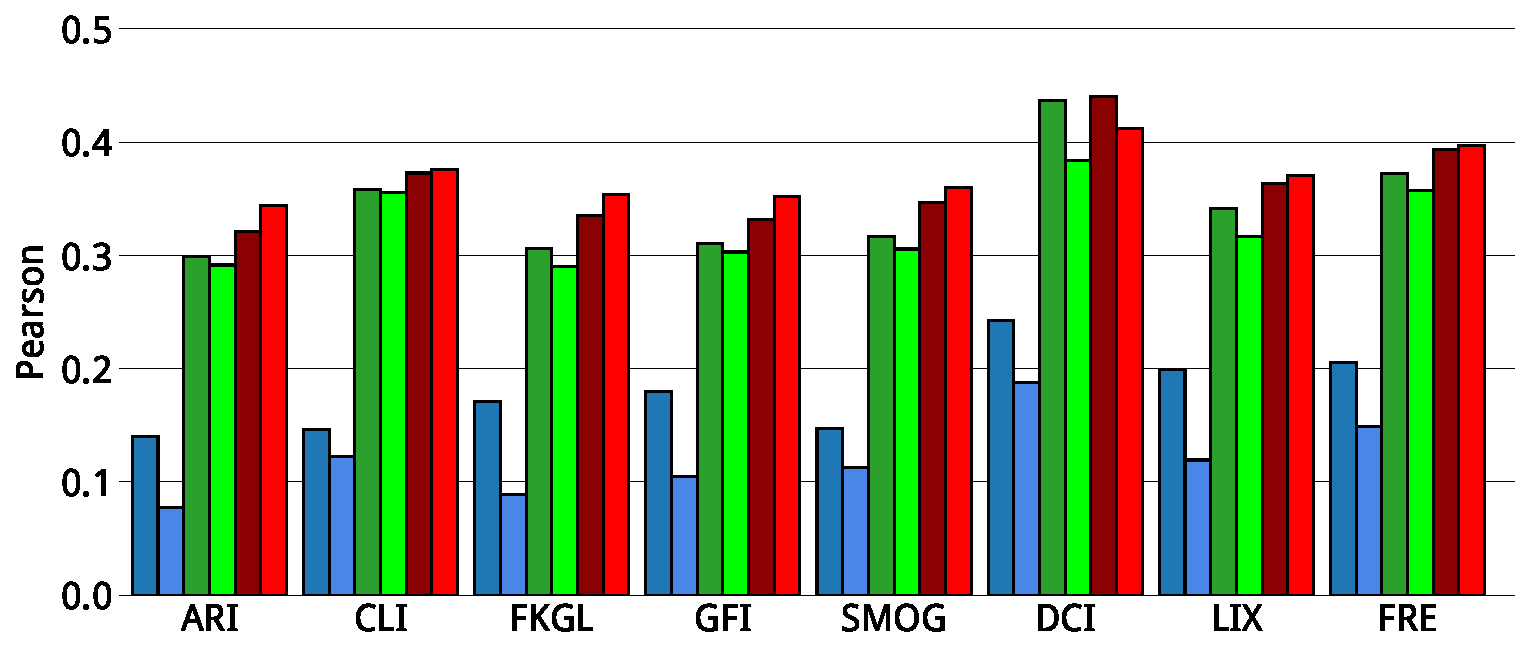
\includegraphics[width=1.\textwidth]{graphics/bar_corr_pearson16_values}
    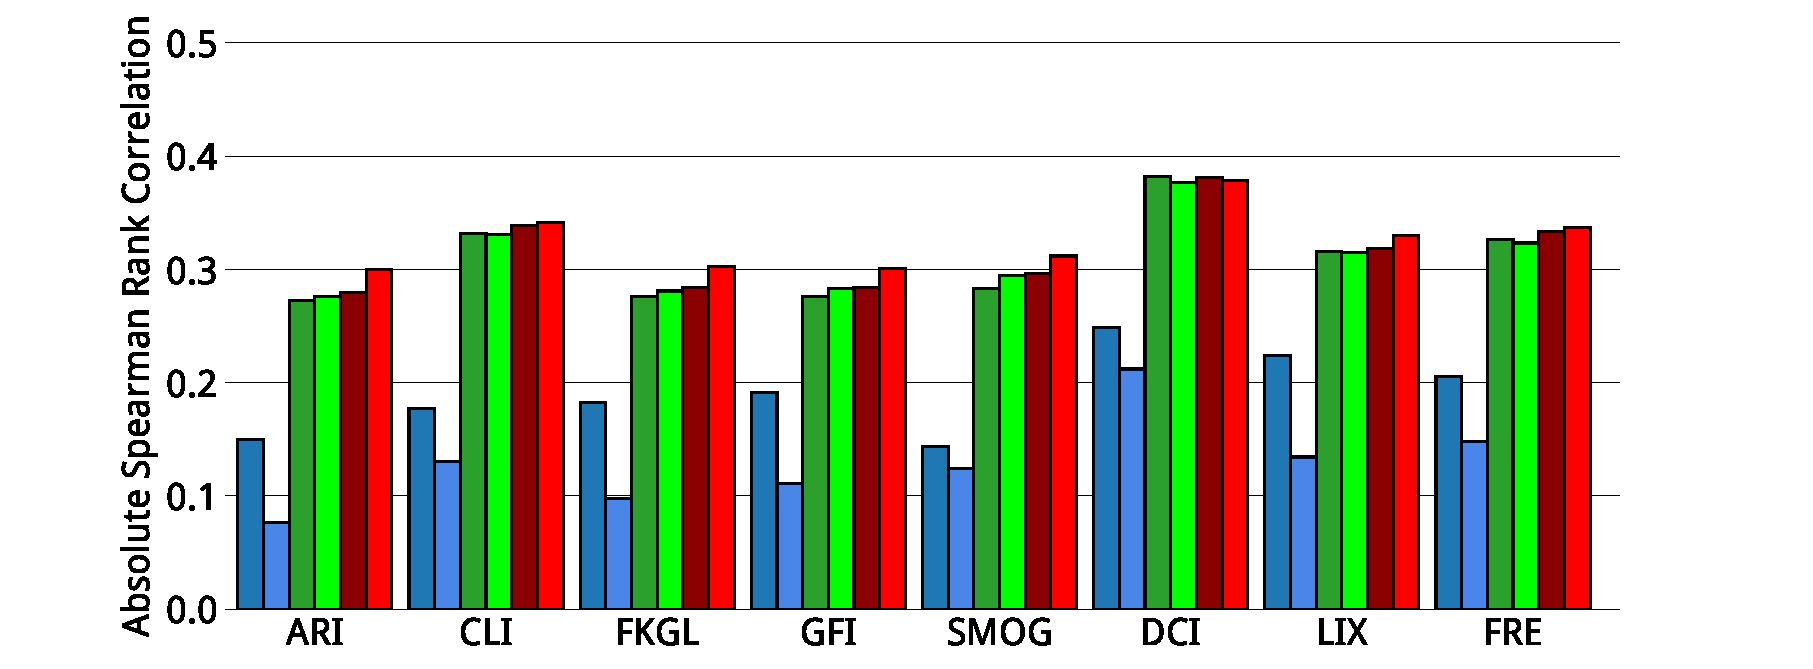
\includegraphics[width=1.\textwidth]{graphics/bar_corr_spearman16_values}
    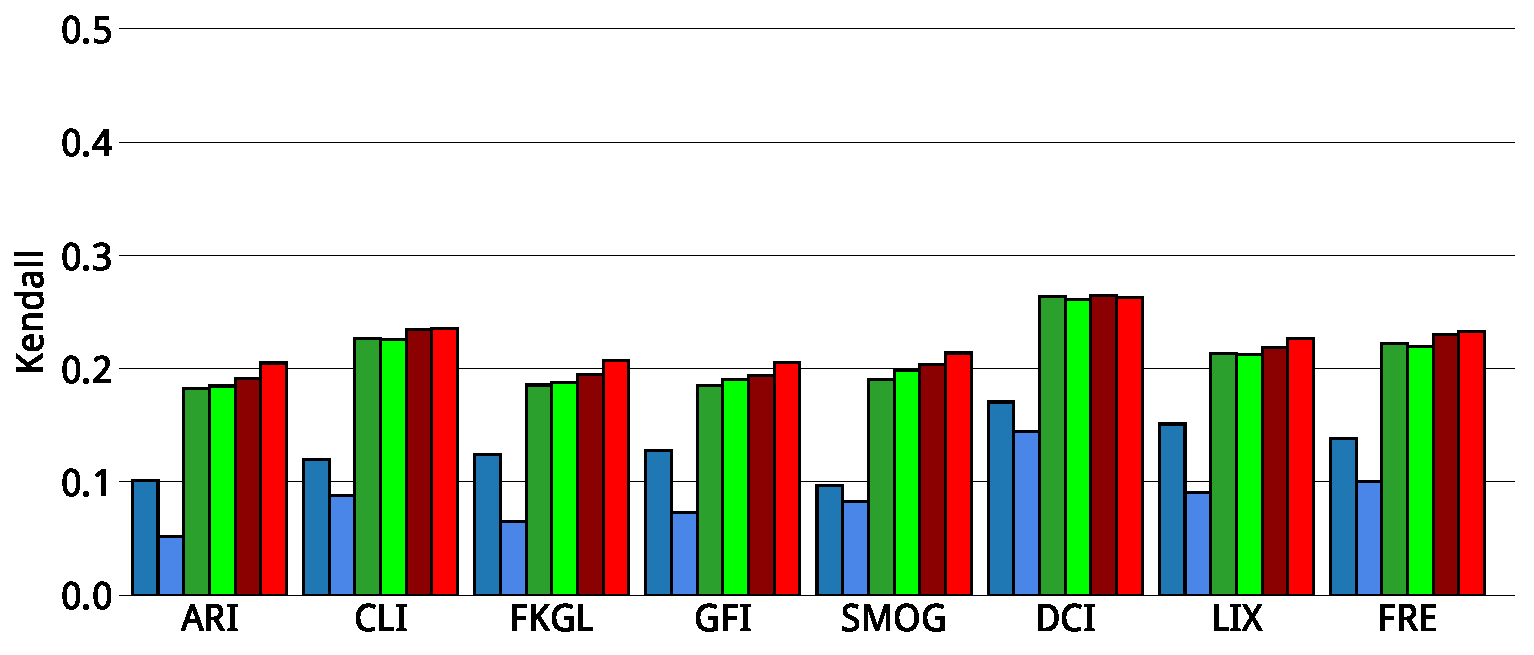
\includegraphics[width=1.\textwidth]{graphics/bar_corr_kendalltau16_values}
    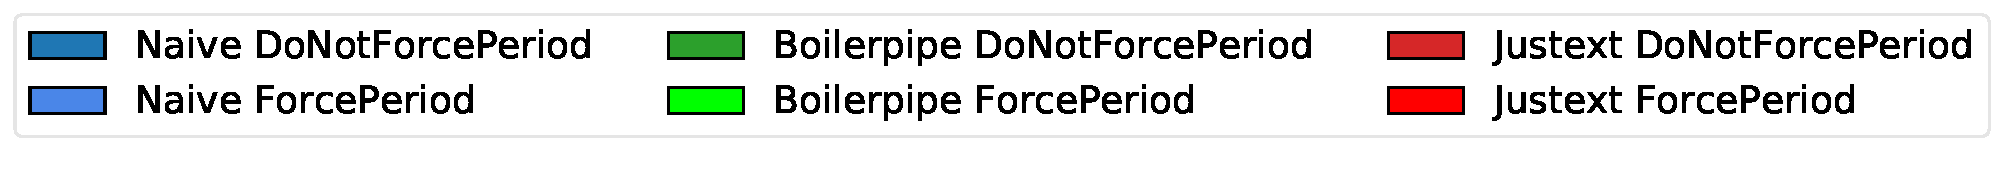
\includegraphics[width=1\textwidth]{graphics/legend62}
    \caption{Correlation of different readability measures and the understandability scores collected in CLEF eHealth 2016.}
   \label{fig:bar_corr_clef16}
\end{figure}


\section{(More) Understandability Estimators}
\label{sec:proxies}

The correlation of readability formulas as shown in Figures~\ref{fig:bar_corr_clef15} and~\ref{fig:bar_corr_clef16} is not strong, with no correlation coefficient being higher than 0.5.
Our next intent is comparing the correlation coefficient of the traditional readability formulas with other methods for understandability estimation, including an evaluation of other humans performing the same task.
For that, we devise and group several methods into semantically related groups which will be following presented.
We summarize all methods in Table~\ref{tab:doc_features}.

%Therefore, what unifies all methods listed in this section is the goal to automatically infer the understandability of a document, in our case, a Web page with medical content.
%For sake of understanding, in Table~\ref{tab:doc_features} we list all the methods used in this chapter to estimate document understandability.
%Note that we divide these estimators into semantically related groups, which are presented below.

\textbf{Traditional Readability Formulas:}
This group contains all the traditional readability formulas listed in Section~\ref{sec:related} (or maybe  in Table~\ref{tab:formulas}).

\textbf{Raw Components of Readability Formulas:}
This group comprises the building blocks that make up the traditional readability measures. Some examples include the average number of characters per word or the average number of syllables in a sentence\footnote{Words were divided into syllables using the Python package Pyphen \url{http://pyphen.org/}}.

\textbf{General Medical Vocabularies:}
This group includes methods such as the number of words with a medical prefix or suffix, i.e. beginning or ending with Latin or Greek particles (e.g., amni-, angi-, algia-, arteri-), acronyms\footnote{The acronym list was obtained from the ADAM database \cite{zhou2006}} or medical vocabularies such as the International Statistical Classification of Diseases and Related Health Problems (ICD), Drugbank and the OpenMedSpel dictionary\footnote{\url{http://extensions.openoffice.org/en/project/openmedspel-en-us}}. 
Methods listed here were matched with documents using a simple keywords matching.

\textbf{Consumer Vocabulary Features:}
the Consumer Health Vocabulary (CHV) is a prominent medical vocabulary dedicated to mapping consumer (layperson) vocabulary to technical terms. 
It attributes a score for each of its concepts with respect to their difficulty, with lower/higher scores for harder/easier concepts.
We used NLM MetaMap\footnote{\url{https://metamap.nlm.nih.gov/}} to map contents occurring in Web documents to the CHV vocabulary.
We further use MetaMap options to also filter only concepts identified as symptoms or diseases.
Similar approach is commonly used in the literature \cite{} \mytodo{maybe cite something that is not ours}.
%The CHV dataset (version 20110204) links part of the UMLS concepts, such as “myocardial infarction”, to everyday expressions, “heart attack”.

\textbf{Expert Vocabulary Features:}
The hierarchy of Medical Subject Headers (MeSH) was previously used in the literature to identify hard concepts, assuming that a concept that is deep in the hierarchy is harder than a shallow one~\cite{yan11}.
As done with CHV, we used MetaMap to map the content of Web documents to MeSH, exploring symptoms and disease concepts separately.

\textbf{Natural Language:}
This group comprises commonly used metrics in the natural language processing field, such as the ratio of part-of-speech (POS) classes, the number of entities in a text, the sentiment polarity and the ratio of words found in English vocabularies. The Python package NLTK 3.2\footnote{\url{http://www.nltk.org/}} was employed for sentiment analysis and POS tagging. The GNU Aspell\footnote{\url{http://www.aspell.net/}} dictionary was used as a standard English vocabulary and a stopword list was built by merging the stopword
lists of the Indri\footnote{\url{http://www.lemurproject.org/indri/}} and Terrier\footnote{\url{http://www.terrier.org/}} toolkits. 

\textbf{HTML Features:}
The aim of this group is to represent a web page by its HTML content.
We hypothesize that a Web page rich of images or with its content well summarized in tables can potentially ease hard subjects such as medicine. 
We identify a large number of HTML tags in this group with the Python library BeautifulSoap v4.4\footnote{\url{https://www.crummy.com/software/BeautifulSoup/}}.

\textbf{Word Frequency Features:}
Common and known words are usually frequent words, while unknown and obscure words are rare. This idea is implemented in readability formulas such as the Dale-Chall index which uses a list of common words and counts the number of words that fall outside this list~\cite{dale48}.
In this work we model word frequency in a straightforward manner: we sort the frequency of all words in a corpus and normalize the ranking of word frequency such that values close to 100 are attributed to common words and values close to 0 to rare words. 
We explore three different corpora in this work:

\begin{itemize}
\item \underline{Medical Reddit:} Reddit\footnote{\url{https://www.reddit.com/}} is an Internet forum with a sizable user community which is responsible for generating its content. Any user can start a discussion receiving replies from any other user. This discussion forum is intensively used for health purposes, for example in the Reddit community AskDocs\footnote{\url{https://www.reddit.com/r/AskDocs/}} licensed nursers and doctors (subject to user identity verification) advise help seekers
        free of charge. We selected six of such communities (medical, AskDocs, AskDoctorSmeeee, Health, WomensHealth, Mens\_Health) and downloaded all user interactions using the Python library PRAW\footnote{\url{https://praw.readthedocs.io/}}. In total 43,018 discussions were collected.

\item \underline{PubMed Central:} PubMed Central\footnote{\url{https://www.ncbi.nlm.nih.gov/pmc/}} is an online digital database of freely available full-text biomedical literature playing a similar role to physicians as the ACM Digital Library does to computer scientists. We used in this work the same collection crafted for the TREC Clinical Decision Support Track 2014 and 2015 (TREC-CDS)\footnote{\url{http://www.trec-cds.org/}} consisting of 733,138 articles. 
 
\item \underline{Medical English Wikipedia:} we filtered articles from a Wikipedia dump\footnote{\url{https://dumps.wikimedia.org/enwiki/}} (May 1st 2017), that contained an Infobox\footnote{A Wikipedia infobox is a template containing structured information that appear on the right of Wikipedia pages to summarize key aspects of concepts} in which at least one of the following words appeared as a property: ICD10, ICD9, DiseasesDB, MeSH, MeSHID, MeshName, MeshNumber, GeneReviewsName, Orphanet, eMedicine, MedlinePlus, drug\_name, Drugs.com, DailyMedID, LOINC.
Figure~\ref{fig:hyperthermia} illustrates a Wikipedia page that is marked as medical because of its Infobox entries.
This idea was successfully implemented in Soldaini et al.~\cite{soldaini15} and our filtering process resulted in a collection of 11,942 articles. 
        Note that this procedure highly favors precision over recall. \mytodo{In case we need space, I suggest we drop this figure}
\end{itemize}

A summary of the statistics of these three collections is reported in Table~\ref{tab:collection_stats}.
In order to calculate word frequency, we removed words that occur less than 5 times in a corpus.
Finally, unless it is explicitly stated otherwise, we ignore out of vocabulary (OV) words in our calculations,

\begin{figure}[th!]
   \centering
   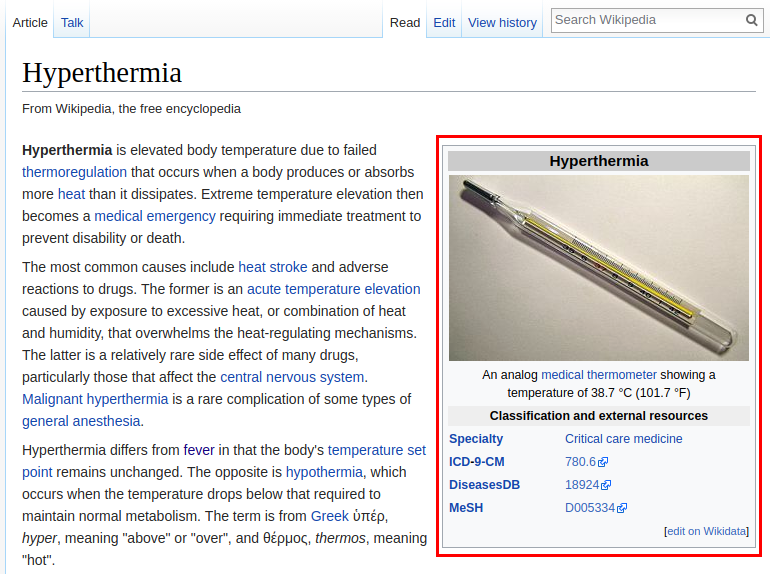
\includegraphics[width=0.50\textwidth]{graphics/hyperthermia}
    \caption{Wikipedia page on hyperthermia. A rectangular red box identify the Infobox on the right hand side containing entries for Specialty, ICD-9-CM, DiseasesDB and MeSH.}
    \label{fig:hyperthermia}
\end{figure}

\begin{table}[!tb]
\centering    
\caption{Statistics for the collections used as background models for understandability estimations.}
\vspace{-0.3cm}
\label{tab:collection_stats}
\resizebox{0.4\textwidth}{!}{
\begin{tabular}{cccc}
\toprule 
\textbf{Statistic} & \textbf{Medical Wikipedia} & \textbf{Medical Reddit} & \textbf{PubMed Central}\tabularnewline
\midrule 
\textbf{Number of Docs.} & 11,868 & 43,019 & 733,191\tabularnewline
\textbf{Number of Words} & 10,655,572 & 11,978,447 & 144,024,976\tabularnewline
\textbf{Number of Unique Words} & 467,650 & 317,106 & 2,933,167\tabularnewline
\textbf{Avg. Words per Doc.} & 898.90 $\pm$ 1351.76 & 278.45 $\pm$ 359.70  & 227.22 $\pm$ 270.44 \tabularnewline
\textbf{Avg. Char per Doc.} & 5107.81 $\pm$ 7618.57  & 1258.44 $\pm$ 1659.96  & 1309.11 $\pm$ 1447.31 \tabularnewline
\textbf{Avg. Char per Word} & 5.68 $\pm$ 3.75  & 4.52 $\pm$ 3.52 &  5.76 $\pm$ 3.51 \tabularnewline
\bottomrule
\end{tabular}
} % End of resizebox
\vspace{-8pt}
\end{table}


\textbf{Machine Learning on Text - Regressors and Classifiers:}
In a recent survey, Kevin Collins-Thompson reports that the future of understandability estimation relies on Machine Learning~\cite{collins2014computational}.
A challenge in using Machine Learning in this task is defining the background corpora used as training set.
A possible setup for our work could have used CLEF 2015 assessments to learn a model for CLEF 2016 and vice-versa, but instead, we opt for a 
more reusable solution for the medical/health domain. 
We employed the three datasets described in Table~\ref{tab:collection_stats} and assume different labels according to the average difficulty of documents in these collections:

\begin{itemize}
    \item Medical Reddit (label 1): Documents in this collection are expected to be written in a colloquial style, and thus the easiest to understand. All the conversations are in fact explicitly directed to assist inexpert health consumers;
    \item Medical English Wikipedia (label 2): Documents in this collection are expected to be less formal than scientific articles, but more formal than a Web forum like Reddit;
    \item PubMed Central (label 3): Documents from this collection are expected to be written in a highly formal style, as the target audience here are physicians, nursers and researchers in the biomedical domain.
\end{itemize}

Models were trained on a Latent Semantic Analysis (LSA) empirically set to have ten dimension based on word counts in documents in these three collections.
We model two different tasks: a classification one and a regression task.
Different labels for the regression could be employed, for example, a label 6 to PubMed Central documents would emphasize that these documents are explicitly made for expert users, being 3 times harder than Wikipedia ones. We did not explore the effects of different labels in this work, it is left as future work.

\begin{table*}[tb]
\caption{Metrics used as understandability proxies; $\star$: raw values are used. $\diamondsuit$: values normalised by number of words in a documents are used. $\dagger$: values normalised by number of sentences in a document are used.}
\label{tab:doc_features}
\resizebox{1.\textwidth}{!}{
\begin{tabular}{llcll}
\cline{1-2} \cline{4-5} 
\textbf{Group} & \textbf{Metric} & \multirow{29}{*}{} & \textbf{Group} & \textbf{Metric}\tabularnewline
\cline{1-2} \cline{4-5} 
\multirow{8}{*}{\textbf{Traditional Readability Formulas}} & Automated Readability Index (ARI) \cite{ari67} &  & \multirow{26}{*}{\textbf{HTML Features}} & \# of Abbr tags\tabularnewline
 & Coleman-Liau Index (CLI) \cite{cli75} &  &  & \# of A tags\tabularnewline
 & Dale Chall Index (DCI) \cite{dale48} &  &  & \# of Blockquote tags\tabularnewline
 & Flesch-Kincaid Grade Level (FKGL) \cite{flesch75} &  &  & \# of Bold tags\tabularnewline
 & Flesch Reading Ease (FRE) \cite{flesch75} &  &  & \# of Cite tags\tabularnewline
 & Gunning Fog Index (GFI) \cite{gunning52} &  &  & \# of Div tags\tabularnewline
 & Lasbarhetsindex (LIX) \cite{lix} &  &  & \# of Forms tags\tabularnewline
 & Simple Measure of Gobbledygook (SMOG) \cite{smog69} &  &  & \# of H1 tags\tabularnewline
\cline{1-2} 
\multirow{10}{*}{\textbf{\makecell{\kern-2.8emRaw Components \\of Readability Measures}}} & \# of Characters $^{\star\diamondsuit\dagger}$ &  &  & \# of H2 tags\tabularnewline
 & \# of Words $^{\star\dagger}$ &  &  & \# of H3 tags\tabularnewline
 & \# of Sentences {$^{\star\diamondsuit}$} &  &  & \# of H4 tags\tabularnewline
 & \# of Difficult Words (Dale Chall list \cite{dale48})
$^{\star\diamondsuit\dagger}$ &  &  & \# of H5 tags\tabularnewline
 & \# of Words Longer than 4 chars $^{\star\diamondsuit\dagger}$ &  &  & \# of H6 tags\tabularnewline
 & \# of Words Longer than 6 chars $^{\star\diamondsuit\dagger}$ &  &  & \# of Hs (any H above)\tabularnewline
 & \# of Words Longer than 10 chars $^{\star\diamondsuit\dagger}$ &  &  & \# of Img tags\tabularnewline
 & \# of Words Longer than 13 chars $^{\star\diamondsuit\dagger}$ &  &  & \# of Input tags\tabularnewline
 & \# of Number of Syllables $^{\star\diamondsuit\dagger}$ &  &  & \# of Link tags\tabularnewline
 & \# of Polysyllable Words (>3 Syllables) $^{\star\diamondsuit\dagger}$ &  &  & \# of DL tags\tabularnewline
\cline{1-2} 
\multirow{6}{*}{\textbf{Medical Vocabularies}} & \# of Words with Medical Prefix $^{\star\diamondsuit\dagger}$ &  &  & \# of UL tags\tabularnewline
 & \# of Words with Medical Suffix $^{\star\diamondsuit\dagger}$ &  &  & \# of OL tags\tabularnewline
 & \# of Acronyms $^{\star\diamondsuit\dagger}$ &  &  & \# of List (DL + UL + OL)\tabularnewline
 & \# of ICD Concepts $^{\star\diamondsuit\dagger}$ &  &  & \# of Q tags\tabularnewline
 & \# of Drugbank $^{\star\diamondsuit\dagger}$ &  &  & \# of Scripts tags\tabularnewline
 & \# of Words in medical dict. (OpenMedSpel) $^{\star\diamondsuit\dagger}$ &  &  & \# of Spans tags\tabularnewline
\cline{1-2} 
    \multirow{6}{*}{\textbf{\makecell{\kern-2.5emConsumer Health\\ Vocabulary (CHV) \cite{zeng06} \\ \kern-6.2emFeatures}}} & CHV Mean Score for all Concepts $^{\star\diamondsuit\dagger}$ &  &  & \# of Table tags\tabularnewline
 & \# of CHV Concepts $^{\star\diamondsuit\dagger}$ &  &  & \# of P tags\tabularnewline
\cline{4-5} 
 & CHV Mean Score for Symptom Concepts $^{\star\diamondsuit\dagger}$ &  & \multirow{20}{*}{\textbf{Word Frequency}} & 25th percentil English Wikipedia\tabularnewline
 & \# of CHV Symptom Concepts $^{\star\diamondsuit\dagger}$ &  &  & 50th percentil English Wikipedia\tabularnewline
 & CHV Mean Score for Disease Concepts $^{\star\diamondsuit\dagger}$ &  &  & 75th percentil English Wikipedia\tabularnewline
 & \# of CHV Disease Concepts $^{\star\diamondsuit\dagger}$ &  &  & Mean Rank English Wikipedia\tabularnewline
\cline{1-2} 
\multirow{6}{*}{\textbf{\makecell{\kern-0.3emMedical Subject\\ Headers (MeSH)}}} & \# of MeSH Concepts $^{\star\diamondsuit\dagger}$ &  &  & Mean Rank English Wikipedia - Includes OV\tabularnewline
 & Average Tree of MeSH Concepts $^{\star\diamondsuit\dagger}$ &  &  & 25th percentil Medical Reddit\tabularnewline
 & \# of MeSH Symptom Concepts $^{\star\diamondsuit\dagger}$ &  &  & 50th percentil Medical Reddit\tabularnewline
 & Average Tree of MeSH Symptom Concepts $^{\star\diamondsuit\dagger}$ &  &  & 75th percentil Medical Reddit\tabularnewline
 & \# of MeSH Disease Concepts $^{\star\diamondsuit\dagger}$ &  &  & Mean Rank Medical Reddit\tabularnewline
 & Average Tree of MeSH Disease Concepts $^{\star\diamondsuit\dagger}$ &  &  & Mean Rank Medical Reddit ncludelude OV\tabularnewline
\cline{1-2} 
\multirow{20}{*}{\textbf{Natural Language}} & Positive Words $^{\star\diamondsuit\dagger}$ &  &  & 25th percentil Pubmed\tabularnewline
 & Negative Words $^{\star\diamondsuit\dagger}$ &  &  & 50th percentil Pubmed\tabularnewline
 & Neutral Words $^{\star\diamondsuit\dagger}$ &  &  & 75th percentil Pubmed\tabularnewline
 & \# of verbs $^{\star\diamondsuit\dagger}$ &  &  & Mean Rank Pubmed\tabularnewline
 & \# of nouns $^{\star\diamondsuit\dagger}$ &  &  &  Mean Rank Pubmed - Includes OV\tabularnewline
 & \# of pronouns $^{\star\diamondsuit\dagger}$ &  &  & 25th p. Wikipedia+Reddit+Pubmed  \tabularnewline
 & \# of adjectives $^{\star\diamondsuit\dagger}$ &  &  & 50th p. Wikipedia+Reddit+Pubmed \tabularnewline
 & \# of adverbs $^{\star\diamondsuit\dagger}$ &  &  & 75th p. Wikipedia+Reddit+Pubmed \tabularnewline
 & \# of adpositions $^{\star\diamondsuit\dagger}$ &  &  & Mean R. Wiki.+Reddit+Pubmed \tabularnewline 
 & \# of conjunctions $^{\star\diamondsuit\dagger}$ & &  & Mean R. Wiki.+Reddit+Pubmed - w. OV \tabularnewline
\cline{4-5} 
 & \# of determiners $^{\star\diamondsuit\dagger}$ & & \multirow{5}{*}{\textbf{Regressor}} & Linear Regressor\tabularnewline  
 & \# of cardinal numbers $^{\star\diamondsuit\dagger}$ &  &  & Gradient Boosting Regressor\tabularnewline
 & \# of particles or other function words $^{\star\diamondsuit\dagger}$ &  &  & Multi-layer Perceptron Regressor\tabularnewline
 & \# of other POS (foreign words, typos) $^{\star\diamondsuit\dagger}$ &  &  & Random Forest Regressor\tabularnewline
 & \# of punctuation $^{\star\diamondsuit\dagger}$ &  &  & Support Vector Machine Regressor\tabularnewline
\cline{4-5} 
 & Height of part-of-speech parser tree $^{\star\diamondsuit\dagger}$ &  &  \multirow{6}{*}{\textbf{Classifier}} & Logistic Regression\tabularnewline
 & \# of Entities $^{\star\diamondsuit\dagger}$ &  &  & Gradient Boosting Classifier\tabularnewline
 & \# of Stopwords $^{\star\diamondsuit\dagger}$ &  &  & Multinomial Naive Bayes\tabularnewline
 & \# of words not found in Aspell Eng. dict. $^{\star\diamondsuit\dagger}$ &  &  & Multi-layer Perceptron Classifier\tabularnewline
 &  &  &  & Random Forest Classifier\tabularnewline
 &  &  &  & Support Vector Machine Classifier\tabularnewline
\cline{1-2} \cline{4-5} 
\end{tabular}
}
\end{table*}


\section{Top Measures from Each Group}
\label{sec:beyond_readability}

We correlated each individual understandability estimator listed in Table~\ref{tab:doc_features} with the human assessments collected in CLEF eHealth 2015 and 2016 campaigns.
We report in Table~\ref{tab:top_corr_metrics} the best metric for each group according to Pearson, Spearman or Kendall correlation.
For some groups, such as the readability formula group, the highest correlated metric was the same for different correlation measure: SMOG Index in CLEF eHealth 2015 and Dale-Chall Index in 2016. 
We highlight the top score value of each correlation measure in each group. Note that there is no single case in which three different metrics were the top correlated for each different correlation measure.
\todo{hypotesis that kendatll tau and spearman always point to the same winner}

Interestingly, Table~\ref{tab:top_corr_metrics} shows that the polysyllable words, best formula component metric for CLEF 2015 data, is the main metric for the SMOG formula, the best readability formula for CLEF 2015. 
Likewise, the number of difficult words, best formula component metric for CLEF 2016, is the main metric for Dale-Chall index, the best readability formula for CLEF 2016.

The top correlation for MeSH group, number of MeSH concepts, reaches much lower correlation than the top correlation metric for the CHV group, the scores of CHV concepts.
The dominating metrics for the Natural Language group are the number of pronouns, the number of stopwords and the number of out of vocabulary words; all these are consistently more correlated than metrics in the MeSH and CHV group.
In turn, the top correlations for the HTML group, counts of P tags and list tags, were the weakest. P tags are used to create paragraphs in a Web page, being roughly a proxy for text lengthiness. 
Top estimators for the word frequency group are based on the Medical Reddit and PubMed counts, with correlations as high as the readability formulas.
Finally, the group with the highest correlated estimators are the regressors and classifiers, with top estimators being the Neural Network regressor and the multinomial Naive Bayes.
\todo{this section misses some sort of conclusion or at least a link to the next section}
%
\begin{table}[t]
\centering    
\caption{Metrics with highest correlation per group. In bold are the metric that archived the highest correlation for a correlation measure.}
\label{tab:top_corr_metrics}
\resizebox{.45\textwidth}{!}{ %%%%
\begin{tabular}{c|c|c|c|c|c|c}
\toprule
\textbf{Dataset} & \textbf{Group} & \textbf{Metric} & \textbf{Preproc.} & \textbf{Pears.} & \textbf{Spear.} & \textbf{Kend.}\tabularnewline
\midrule
\multirow{15}{*}{CLEF 2015} & RF & SMOG Index & JST NFP & \textbf{0.438} & \textbf{0.388} & \textbf{0.286}\tabularnewline
\cmidrule{2-7} 
 & \multirow{2}{*}{CRF} & Avg. Num. of Polysyl. Words per Word & JST FP & \textbf{0.429} & 0.364 & 0.268\tabularnewline
 &  & Avg. N. of Polysyl. Words per Sentence & JST NFP & 0.192 & \textbf{0.388} & \textbf{0.286}\tabularnewline
\cmidrule{2-7} 
& \multirow{2}{*}{GMV} & Avg. N. Medical Prefixes per Word & Naive FP & \textbf{0.314} & 0.312 & 0.229\tabularnewline
 &  & Number of Medical Prefixes & Naive FP & 0.131 & \textbf{0.368} & \textbf{0.272}\tabularnewline
\cmidrule{2-7} 
 & CMV & CHV Mean Score for all Concepts & Naive FP & \textbf{0.371} & \textbf{0.314} & \textbf{0.228}\tabularnewline
\cmidrule{2-7} 
 & EMV & Number of MeSH Concepts & Naive FP & \textbf{0.227} & \textbf{0.249} & \textbf{0.178}\tabularnewline
\cmidrule{2-7} 
 &  \multirow{2}{*}{NLF} & N. of words not found in Aspell Dict. & JST NFP & \textbf{0.351} & 0.276 & 0.203\tabularnewline
 &  & Number of Pronouns per Word & Naive FP & 0.271 & \textbf{0.441} & \textbf{0.325}\tabularnewline
\cmidrule{2-7} 
 & HF & Number of P Tags & None & \textbf{0.219} & \textbf{0.196} & \textbf{0.142}\tabularnewline
\cmidrule{2-7} 
 &  \multirow{2}{*}{WFF} & Mean Rank Medical Reddit - Includes OV & JST NFP & \textbf{0.435} & 0.277 & 0.197\tabularnewline
 &  & 25th percentil Pubmed & JST NFP & 0.330 & \textbf{0.347} & \textbf{0.256}\tabularnewline
\cmidrule{2-7} 
 &  \multirow{2}{*}{MLR} & Neural Network Regressor & BOI NFP & \textbf{0.602} & 0.394 & 0.287\tabularnewline
 &  & Neural Network Regressor & JST FP & 0.565 & \textbf{0.438} & \textbf{0.324}\tabularnewline
\cmidrule{2-7} 
 & MLC & Multinomial Naive Bayes & Naive FP & \textbf{0.573} & \textbf{0.477} & \textbf{0.416}\tabularnewline
\midrule
\midrule
\multirow{18}{*}{CLEF 2016} & \multirow{2}{*}{RF} & Dale Chall Index & JST FP & \textbf{0.439} & 0.381 & 0.264\tabularnewline
 &  & Dale Chall Index & BOI FP & 0.437 & \textbf{0.382} & \textbf{0.264}\tabularnewline
\cmidrule{2-7} 
 & CRF & Avg. Difficult Words Per Word & BOI FP & \textbf{0.431} & \textbf{0.379} & \textbf{0.262}\tabularnewline
\cmidrule{2-7} 
 & \multirow{2}{*}{GMV} & Avg. Prefixes per Sentence & JST FP & \textbf{0.263} & 0.242 & 0.164\tabularnewline
 &  & ICD Concepts Per Sentence & JST NFP & 0.014 & \textbf{0.253} & \textbf{0.172}\tabularnewline
\cmidrule{2-7} 
 & \multirow{2}{*}{CMV} & CHV Mean Score for all Concepts & JST FP & \textbf{0.329} & 0.313 & 0.216\tabularnewline
 &  & CHV Mean Score for all Concepts & BOI FP & 0.329 & \textbf{0.325} & \textbf{0.224}\tabularnewline
\cmidrule{2-7} 
 & \multirow{2}{*}{EMV} & Number of MeSH Concepts & BOI NFP & \textbf{0.201} & 0.166 & 0.113\tabularnewline
 &  & Number of MeSH Disease Concepts & BOI NFP & 0.179 & \textbf{0.192} & \textbf{0.132}\tabularnewline
\cmidrule{2-7} 
 & \multirow{2}{*}{NLF} & Avg. Stopword Per Word & BOI FP & \textbf{0.344} & 0.312 & 0.213\tabularnewline
 &  & Number of Pronouns & BOI FP & 0.341 & \textbf{0.364} & \textbf{0.252}\tabularnewline
\cmidrule{2-7} 
& \multirow{2}{*}{HF} & Number of Lists & \multirow{2}{*}{None} & \textbf{0.114} & 0.021 & 0.015\tabularnewline
 &  & Number of P Tags &  & 0.110 & \textbf{0.123} & \textbf{0.084}\tabularnewline
\cmidrule{2-7} 
 & \multirow{2}{*}{WFF} & Mean Rank Medical Reddit & BOI NFP & \textbf{0.387} & 0.312 & 0.214\tabularnewline
 &  & 50th percentil Medical Reddit & JST NFP & 0.351 & \textbf{0.315} & \textbf{0.216}\tabularnewline
\cmidrule{2-7} 
 & \multirow{2}{*}{MLR} & Neural Network Regressor & JST NFP & \textbf{0.454} & \textbf{0.373} & 0.258\tabularnewline
 &  & Random Forest Regressor & BOI NFP & 0.389 & 0.355 & \textbf{0.264}\tabularnewline
\cmidrule{2-7} 
 & MLC & Multinomial Naive Bayes & JST FP & \textbf{0.461} & \textbf{0.391} & \textbf{0.318}\tabularnewline
\bottomrule
\end{tabular}
} %%%%% ---- 
\end{table}

%

\section{Which Preprocessing Approach To Prefer}
\label{sec:which_preprocessing}

We further investigate the preprocessing steps with the groups of features introduced in Table~\ref{tab:doc_features}.
For that, we present in Figures~\ref{fig:boxplot_corr_docs_2015} and~\ref{fig:boxplot_corr_docs_2016} the box plot of different correlation metrics divided by preprocessing alternative for CLEF eHealth 2015 and 2016. 
For instance, the very first box plot in the upper part of these figures shows the absolute Pearson's rank correlation of different readability metrics when using a combination of Naive and ForcePeriod as preprocessing steps.
Boxes extend from the lower to upper quartile values of the data, with a line at the median. Whiskers extend from the box to show the range of the data. Flier points are those past the end of the whiskers, usually interpreted as outlier values.

We also include in Figures~\ref{fig:boxplot_corr_docs_2015} and~\ref{fig:boxplot_corr_docs_2016} boxes for the summary of the 3 preprocessing procedures to remove HTML, the use of HTML features, which is done without any preprocessing and the comparison with other human assessors. For CLEF eHealth 2015, we used as human assessments the additional assessments made by unpaid medical students and health consumers (see~\cite{palotti16b}), while for CLEF eHealth 2016 data, we randomly selected 100 pages that were assessed by another assessor. \mytodo{add at least another person doing assessments}.
The correlations with human assessments provide important insights on how hard and subjective understandability assessments are.

\begin{figure}[th!]
   \centering
   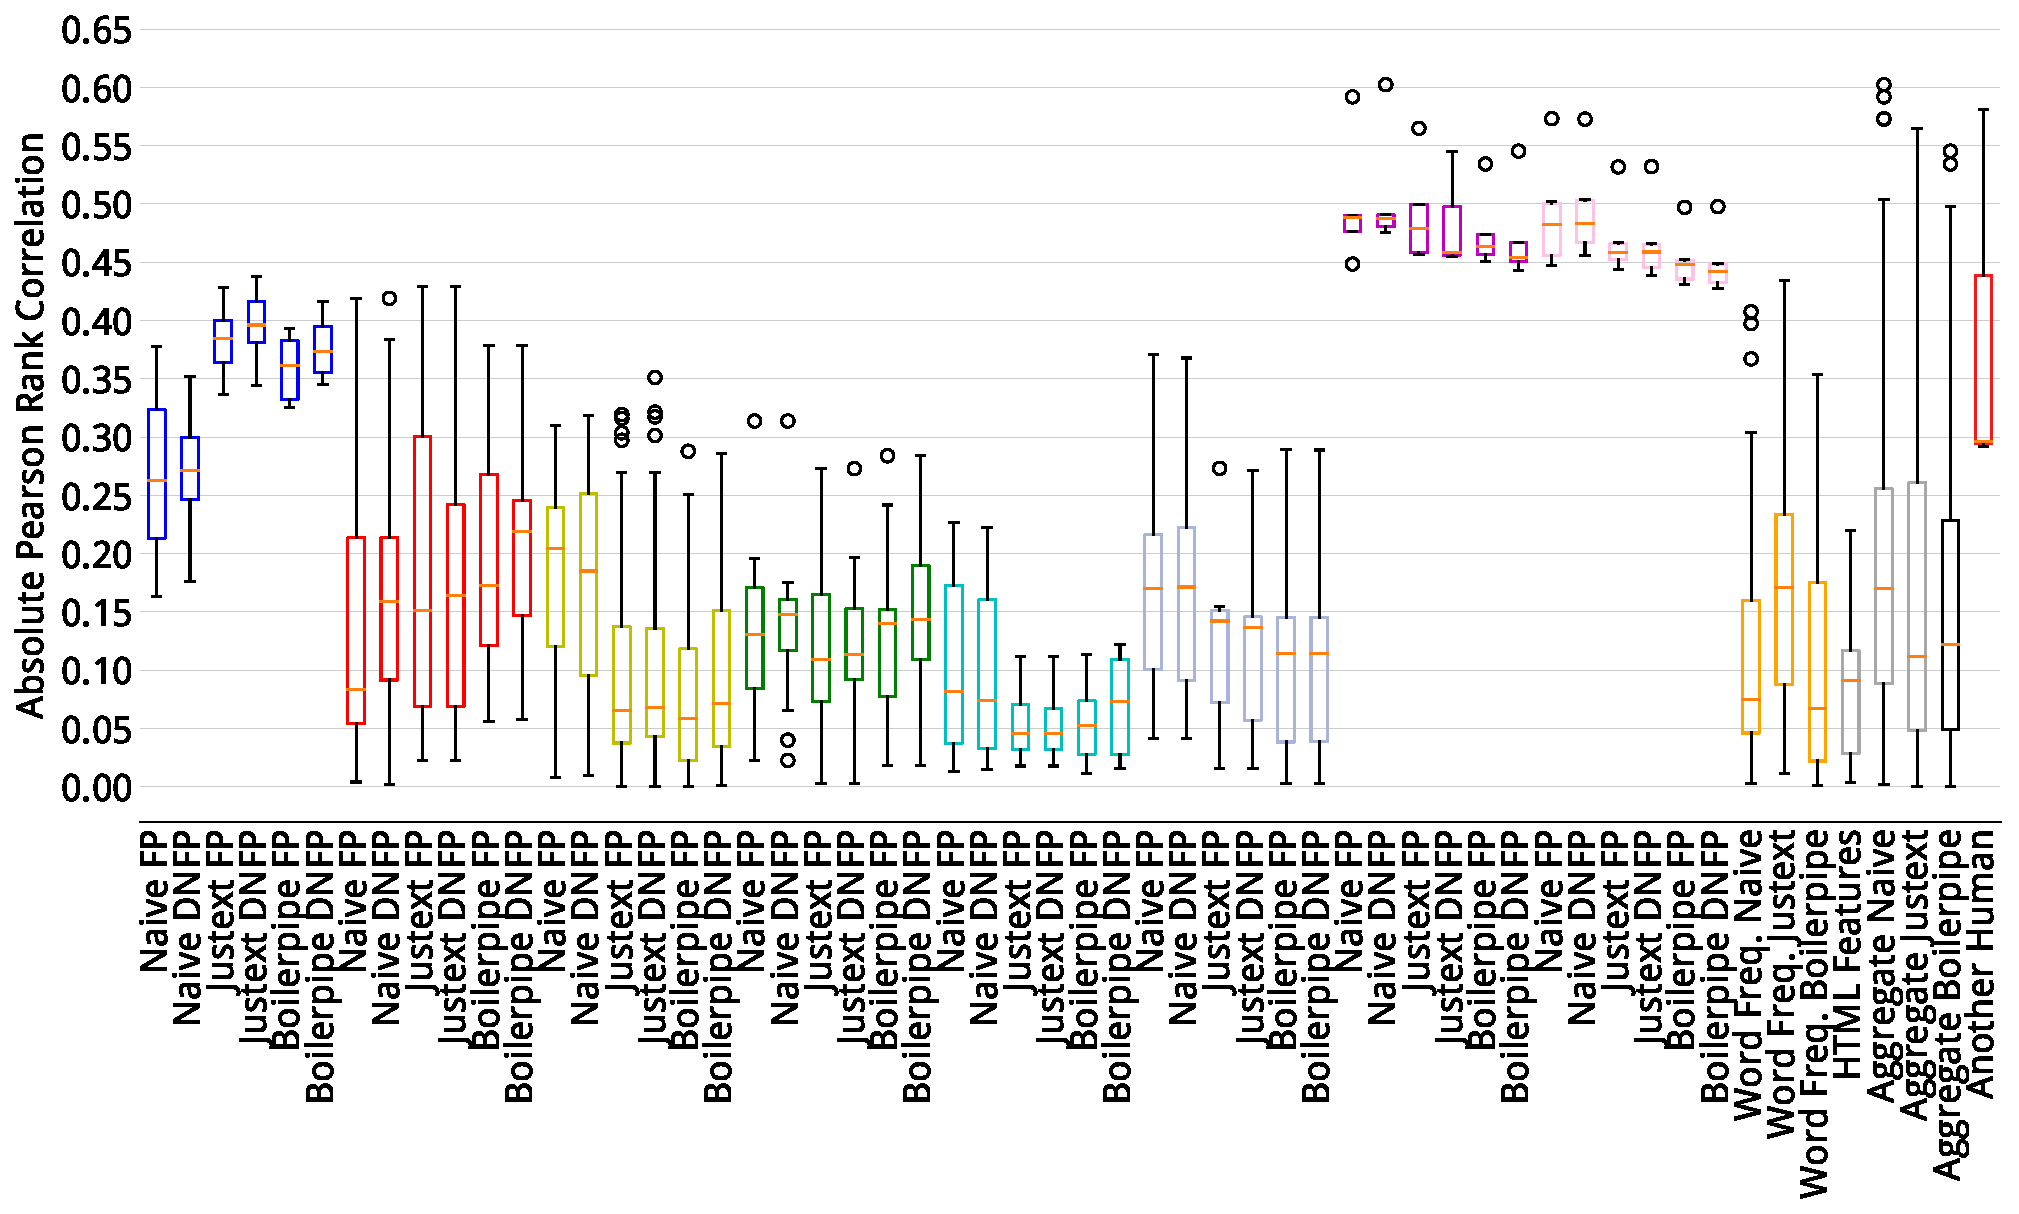
\includegraphics[width=0.70\textwidth]{graphics/box_pearson15_raw_values}
   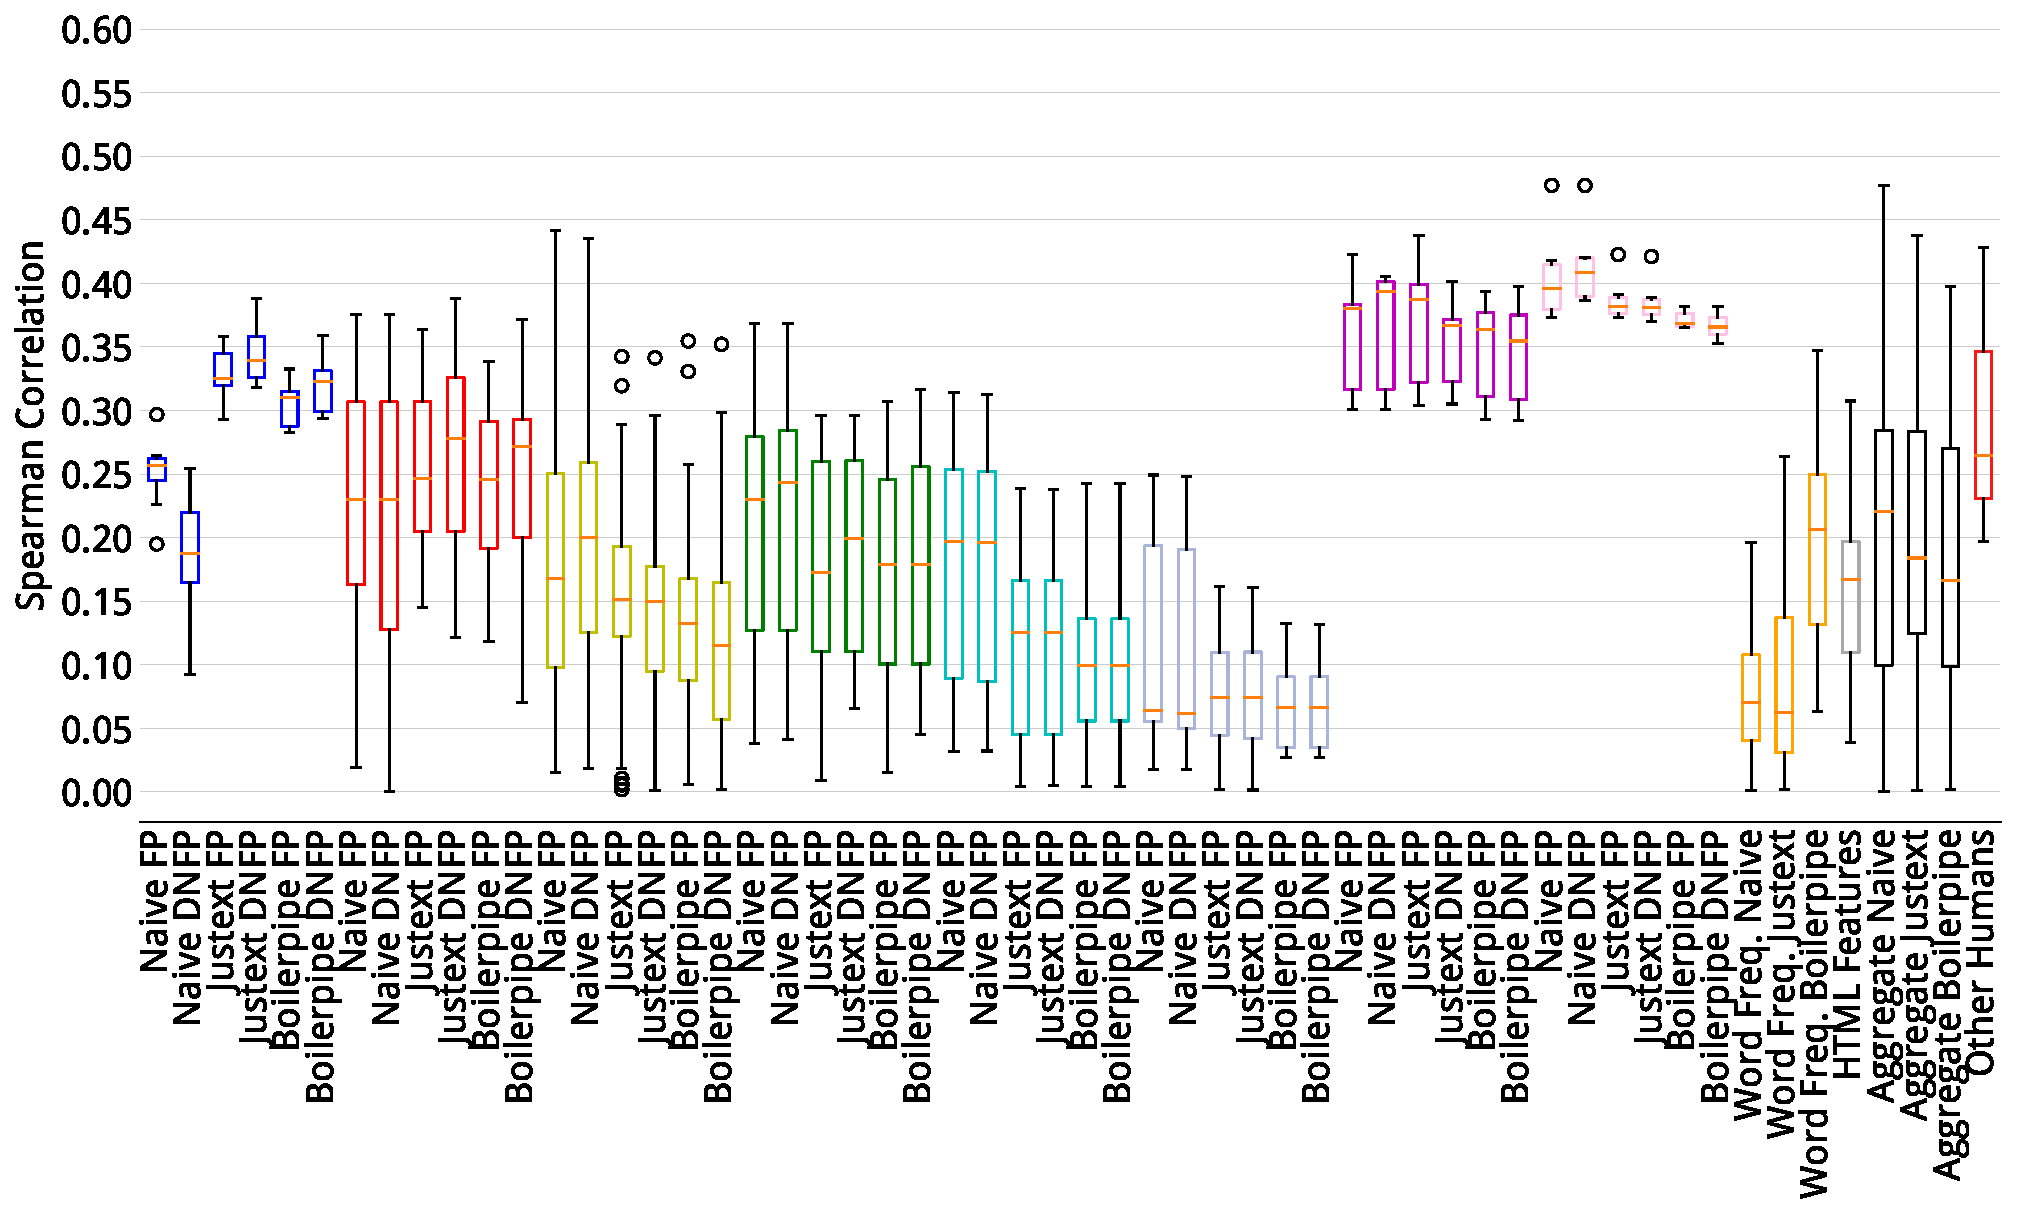
\includegraphics[width=0.70\textwidth]{graphics/box_spearman15_raw_values}
   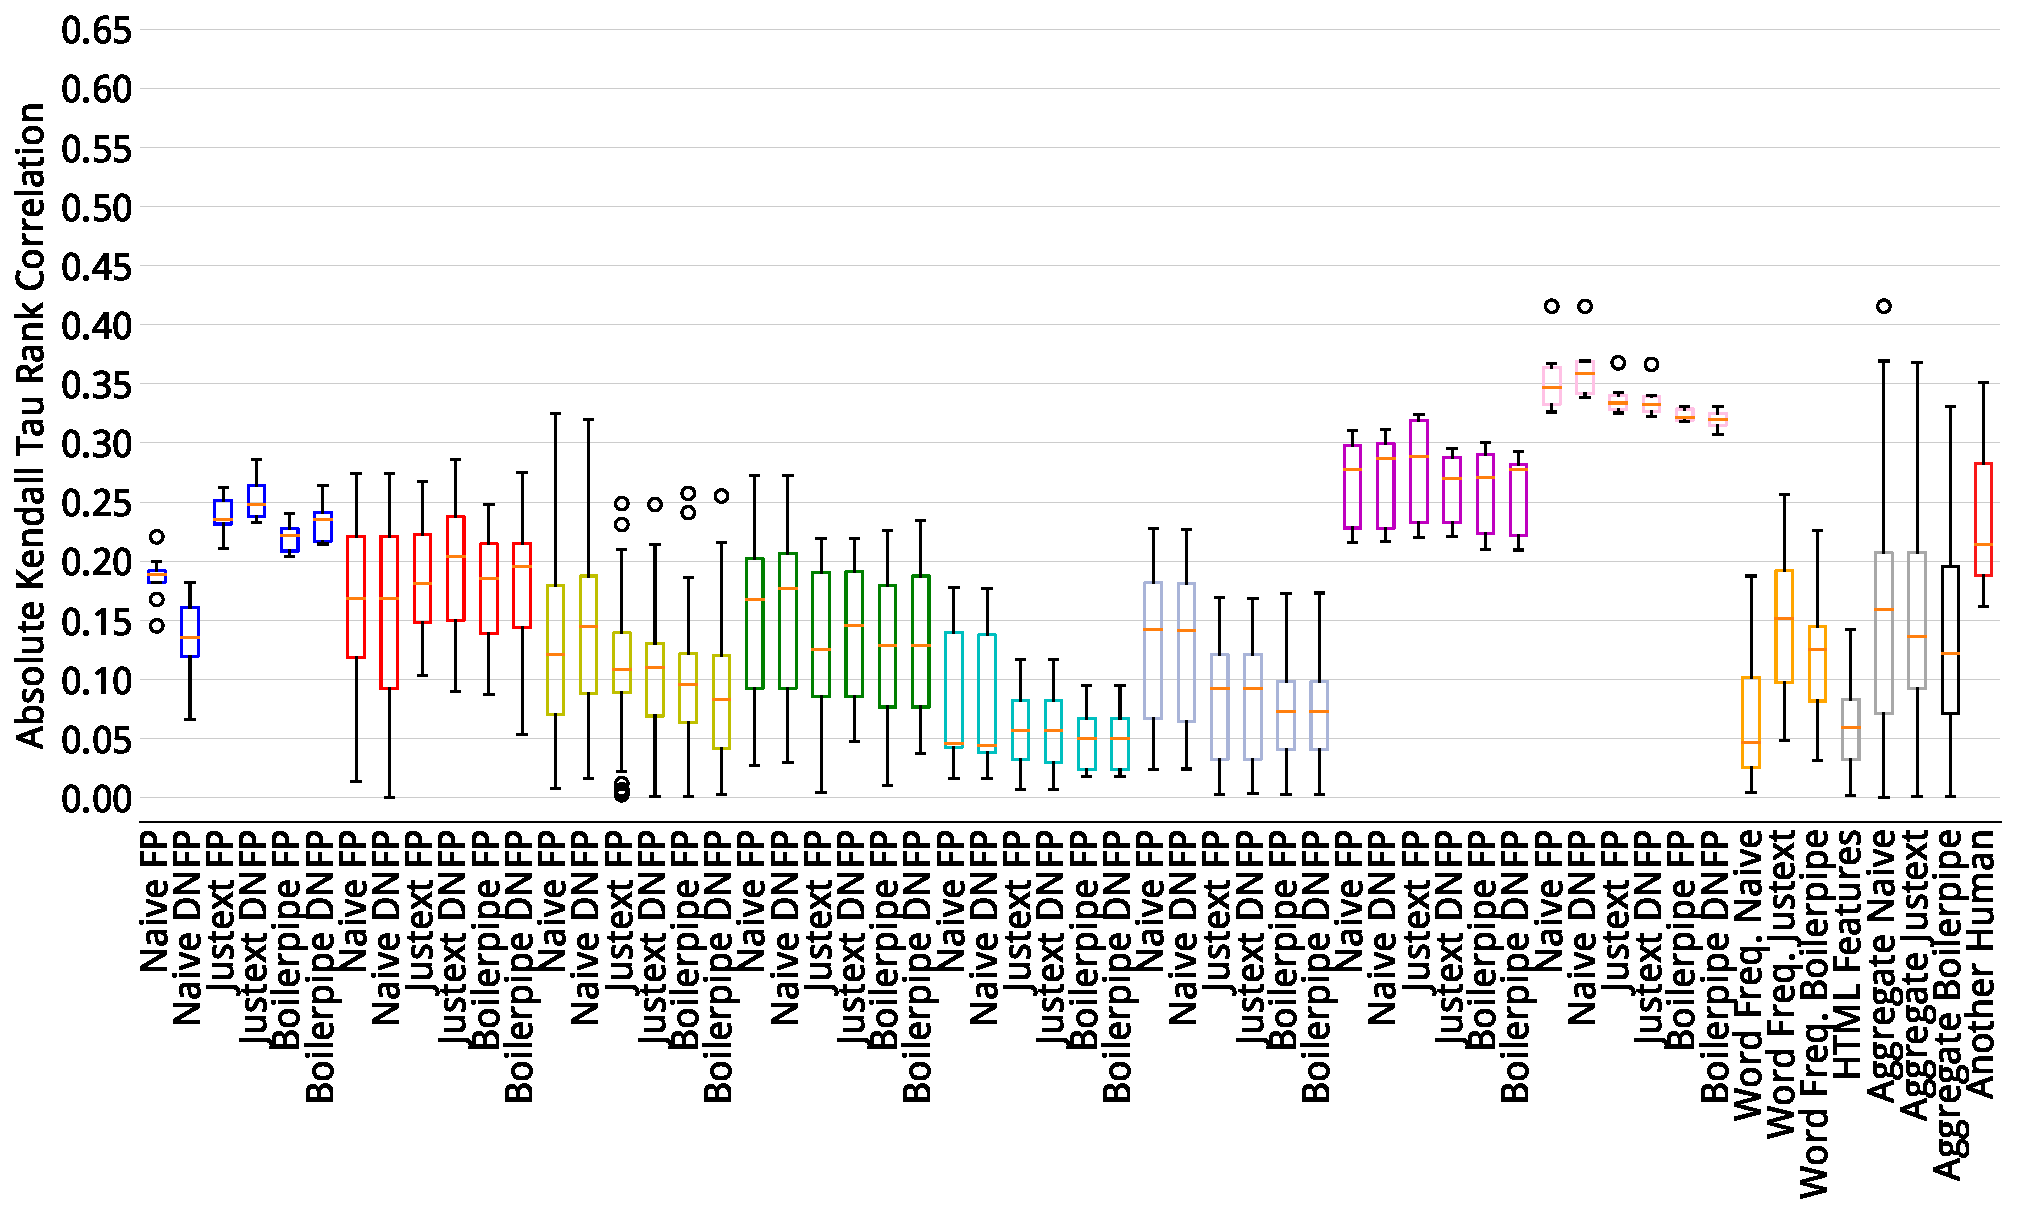
\includegraphics[width=0.70\textwidth]{graphics/box_kendalltau15_raw_values}
    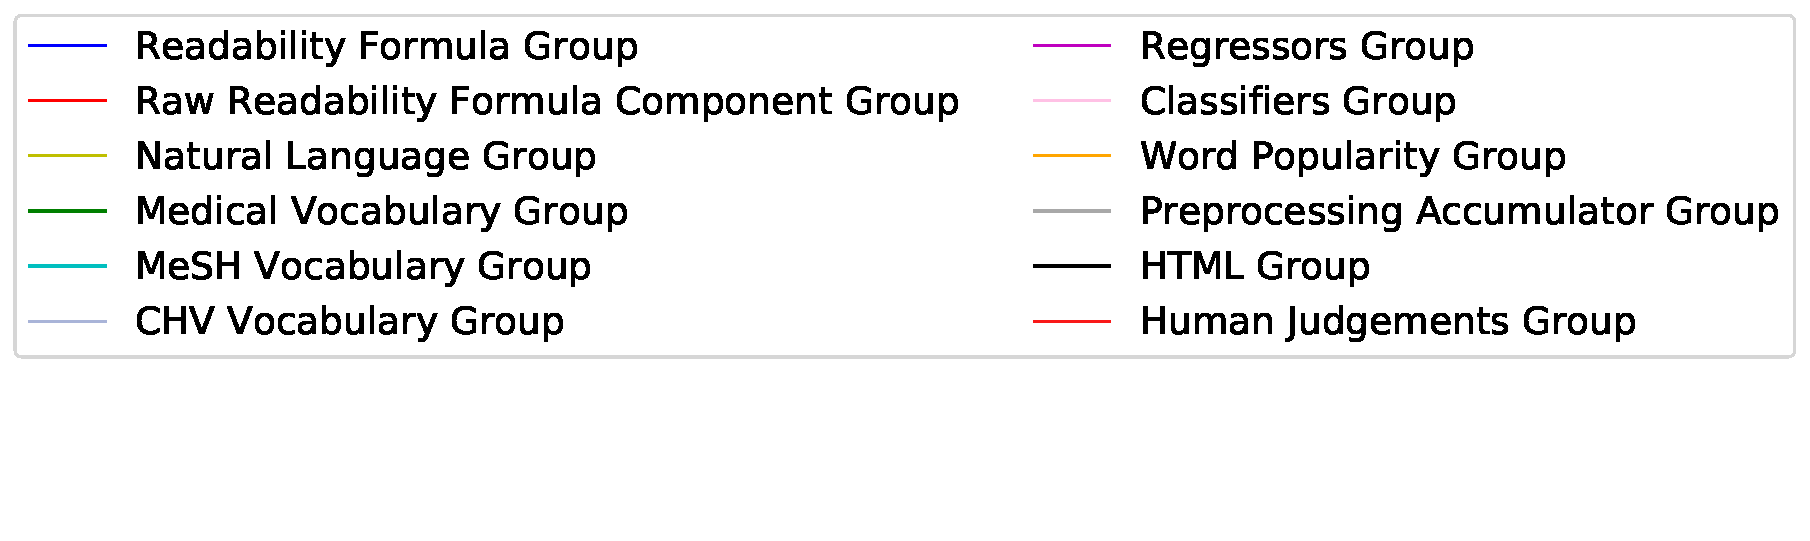
\includegraphics[width=0.65\textwidth]{graphics/legendCorr}
    \vspace{-1.cm}
    \caption{Box plots divided by feature groups. Correlations are calculated using understandability labels from relevant documents assessed in CLEF eHealth 2015}
   \label{fig:boxplot_corr_docs_2015}
\end{figure}

\begin{figure}[th!]
   \centering
   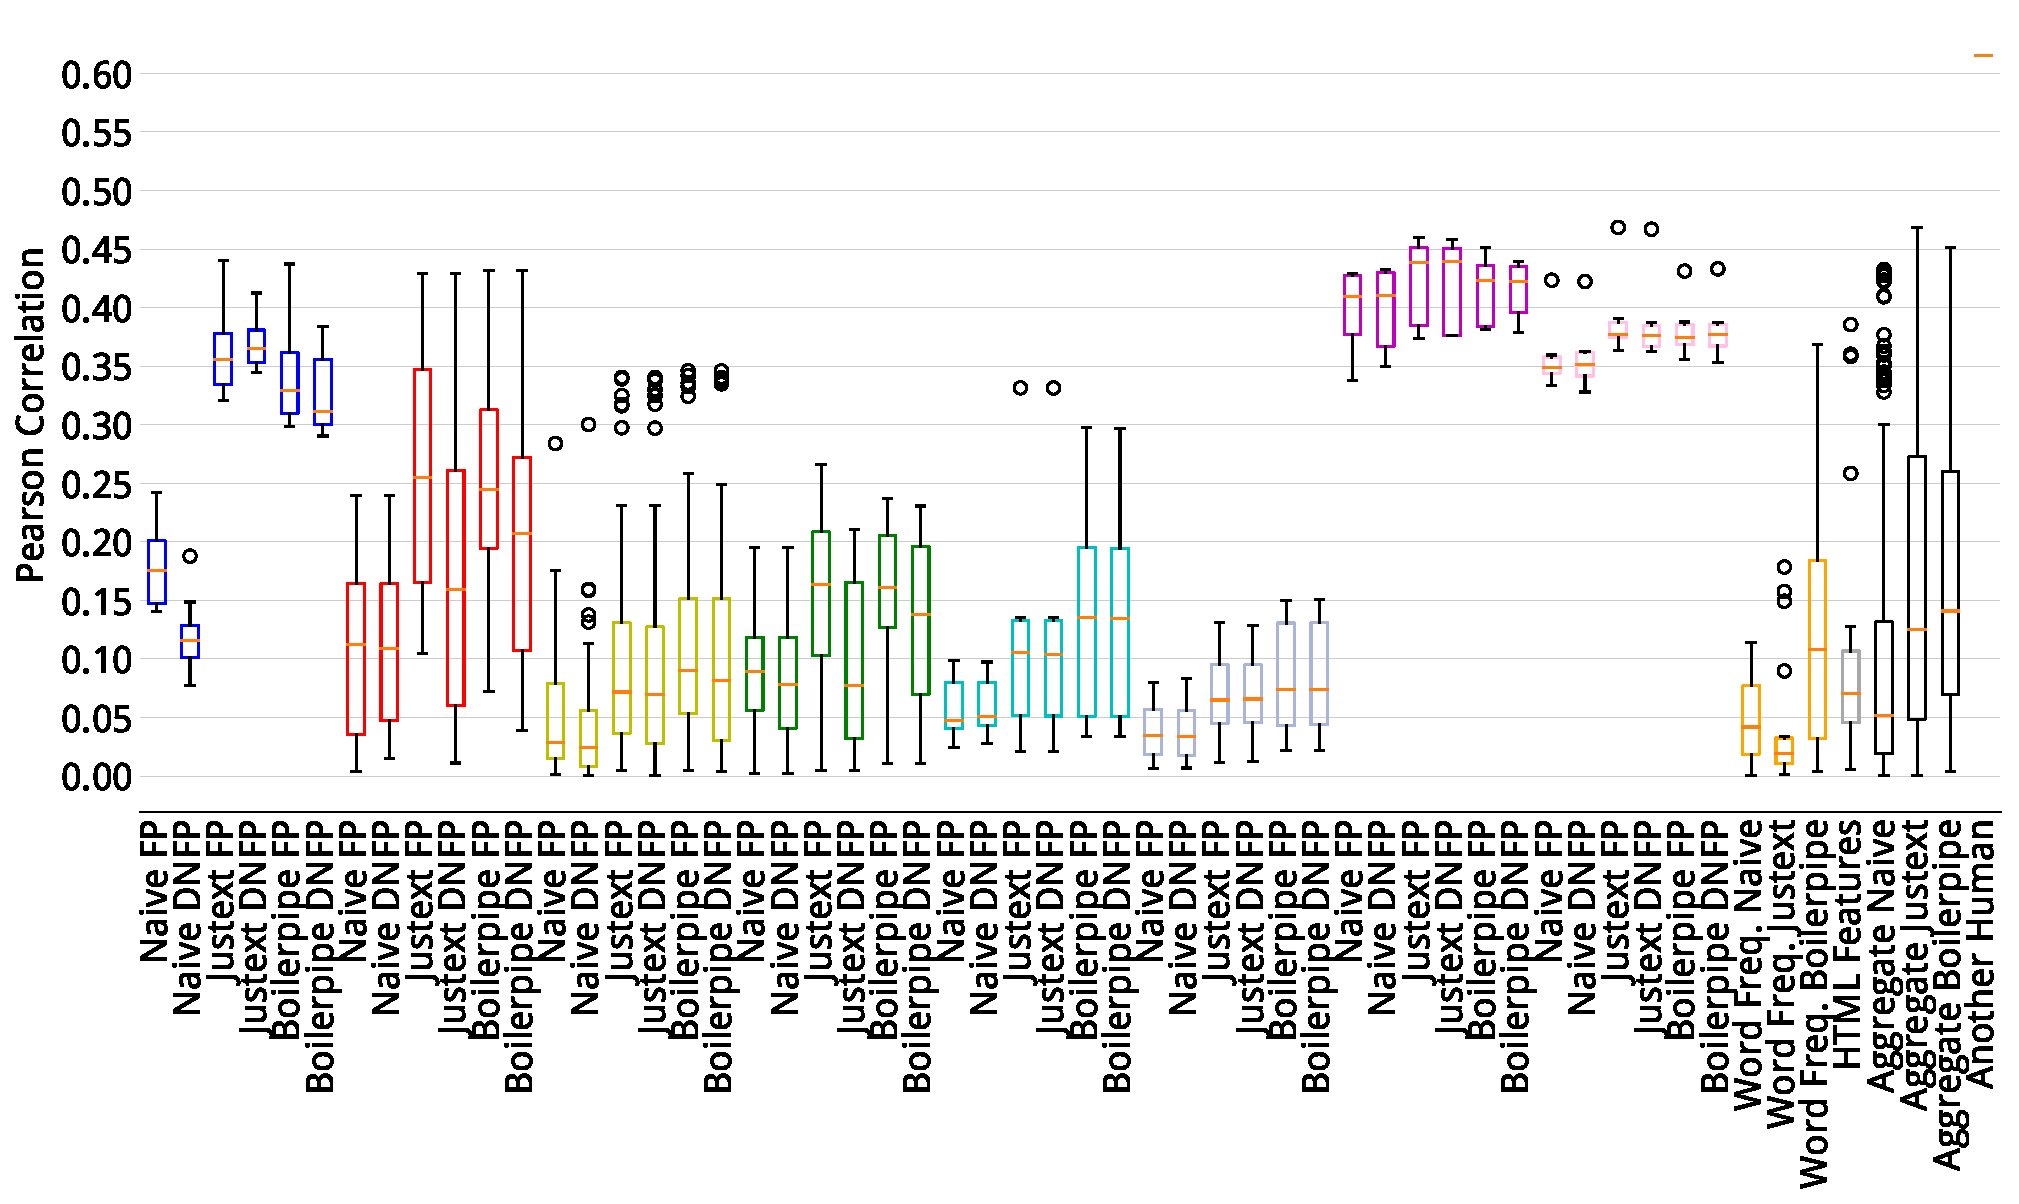
\includegraphics[width=0.70\textwidth]{graphics/box_pearson16_raw_values}
   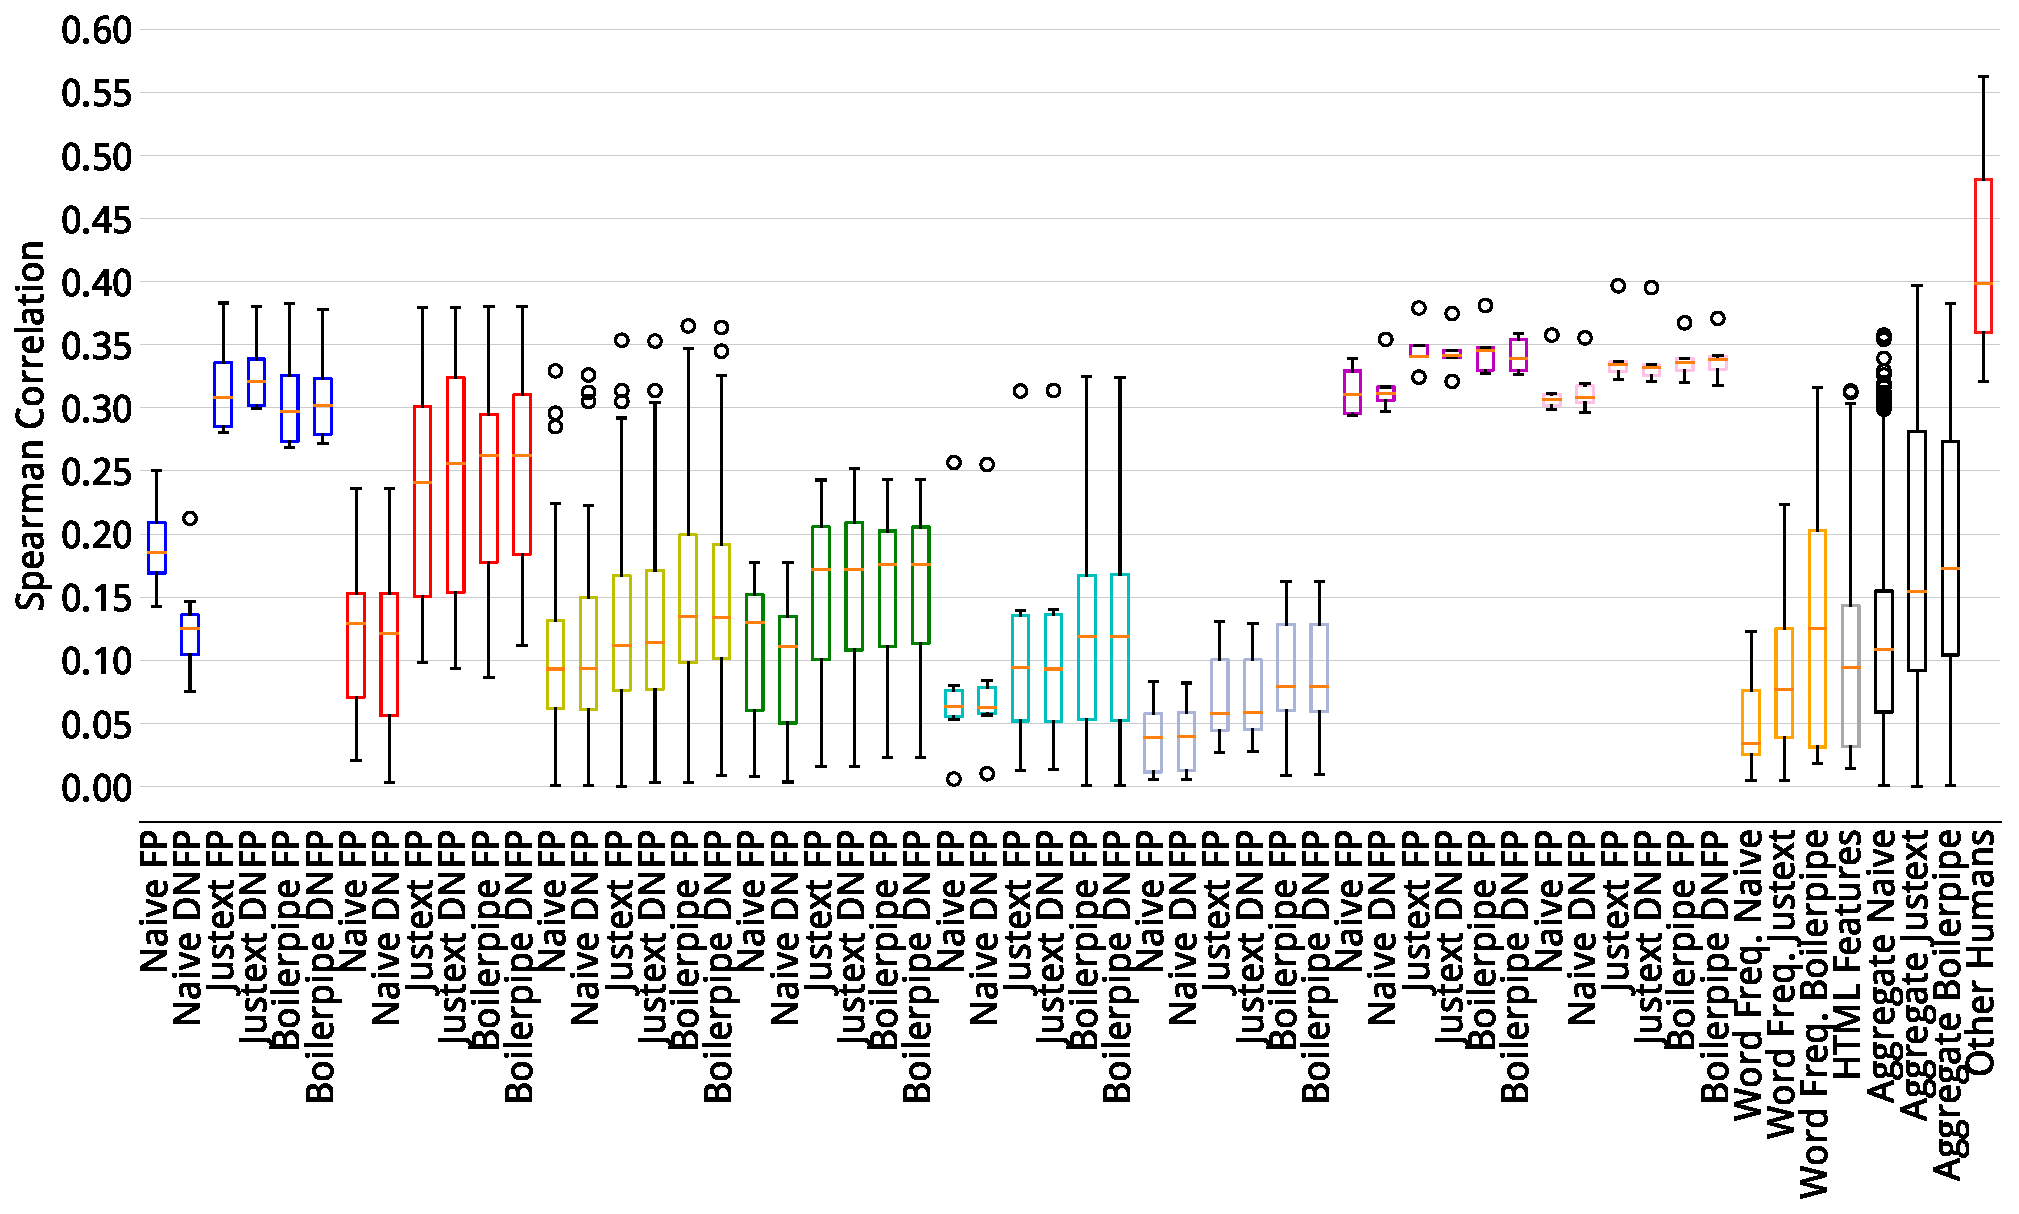
\includegraphics[width=0.70\textwidth]{graphics/box_spearman16_raw_values}
   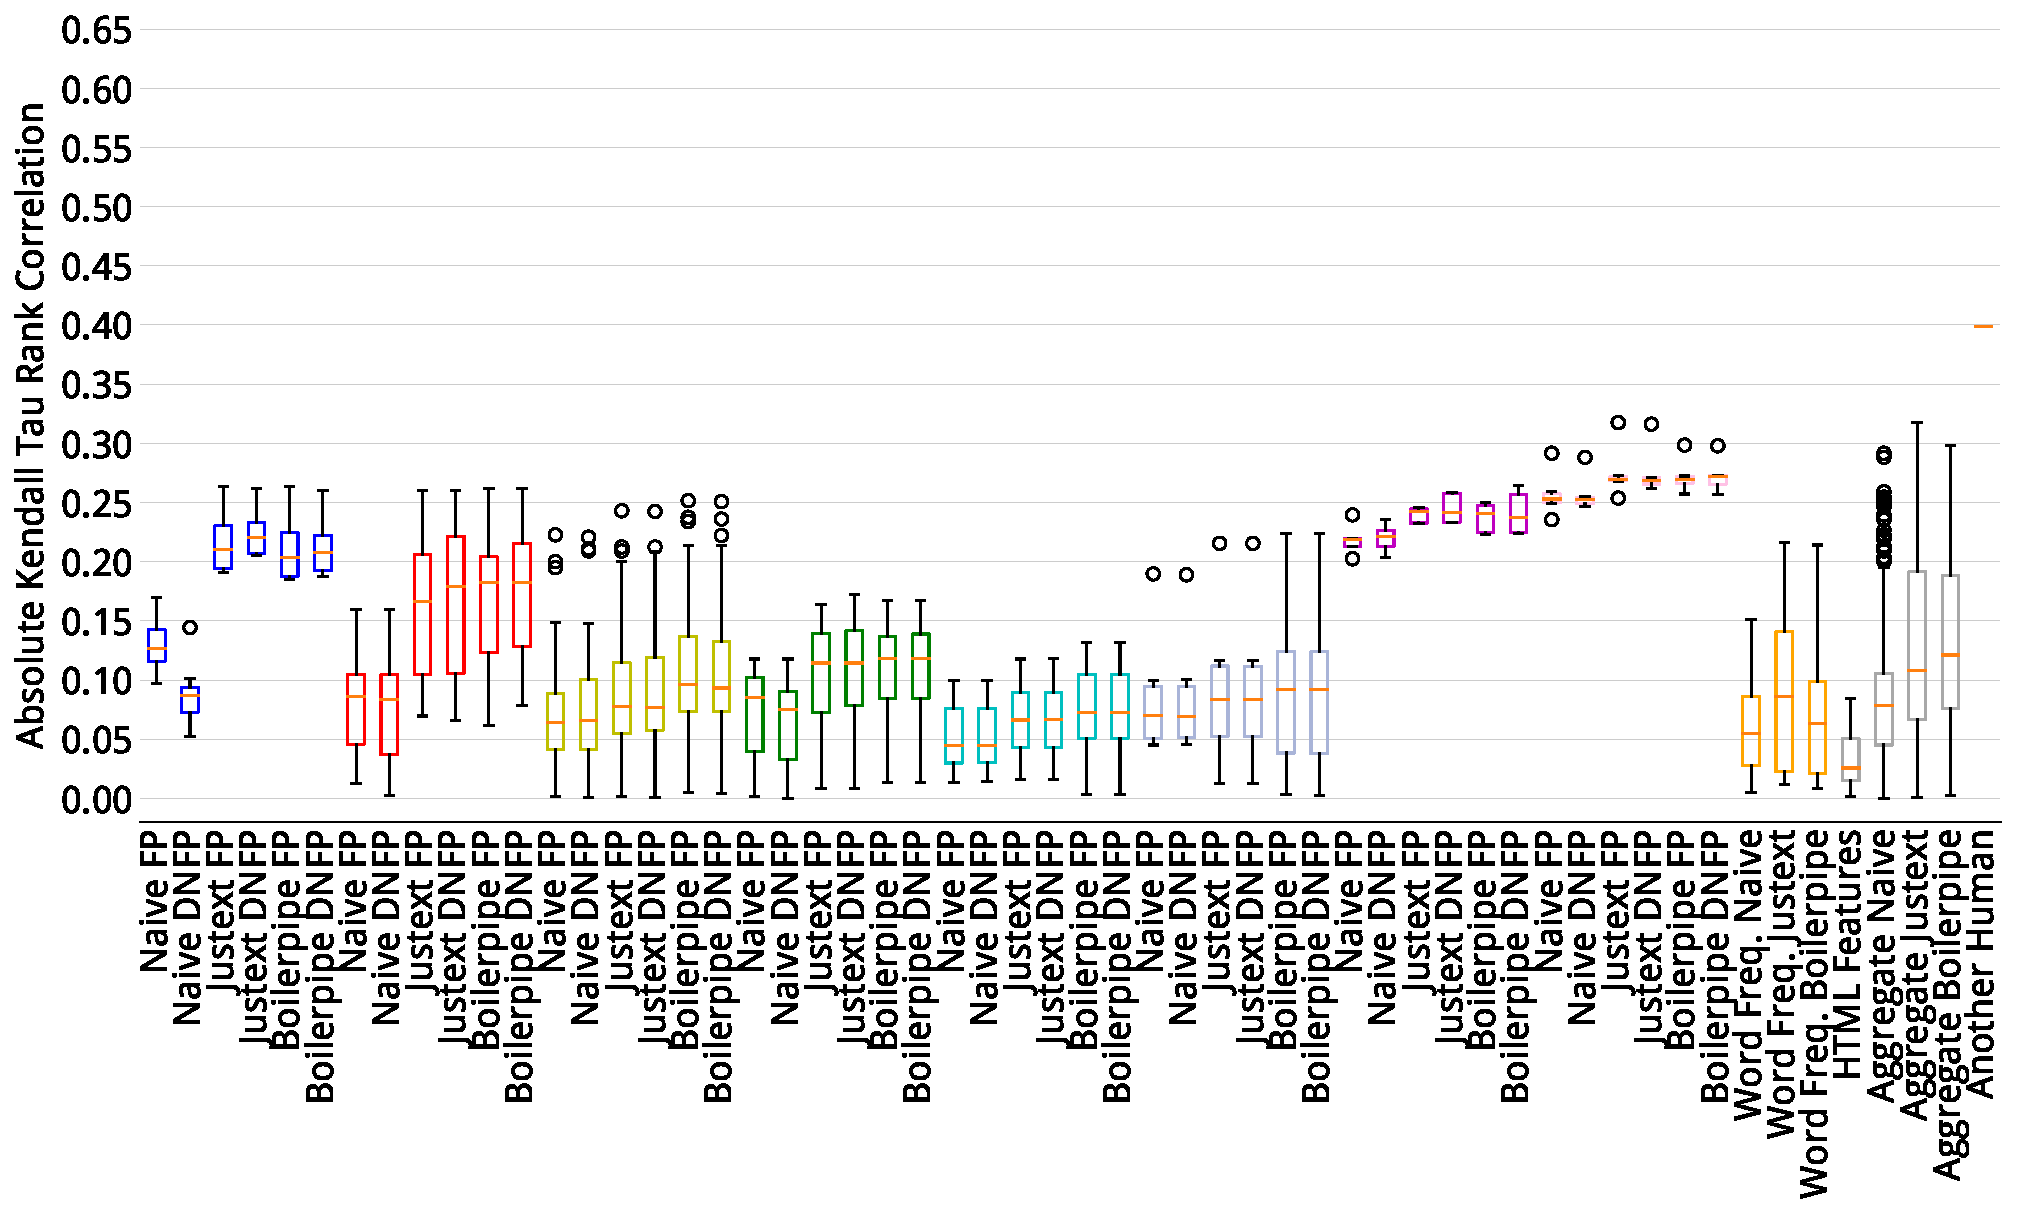
\includegraphics[width=0.70\textwidth]{graphics/box_kendalltau16_raw_values}
    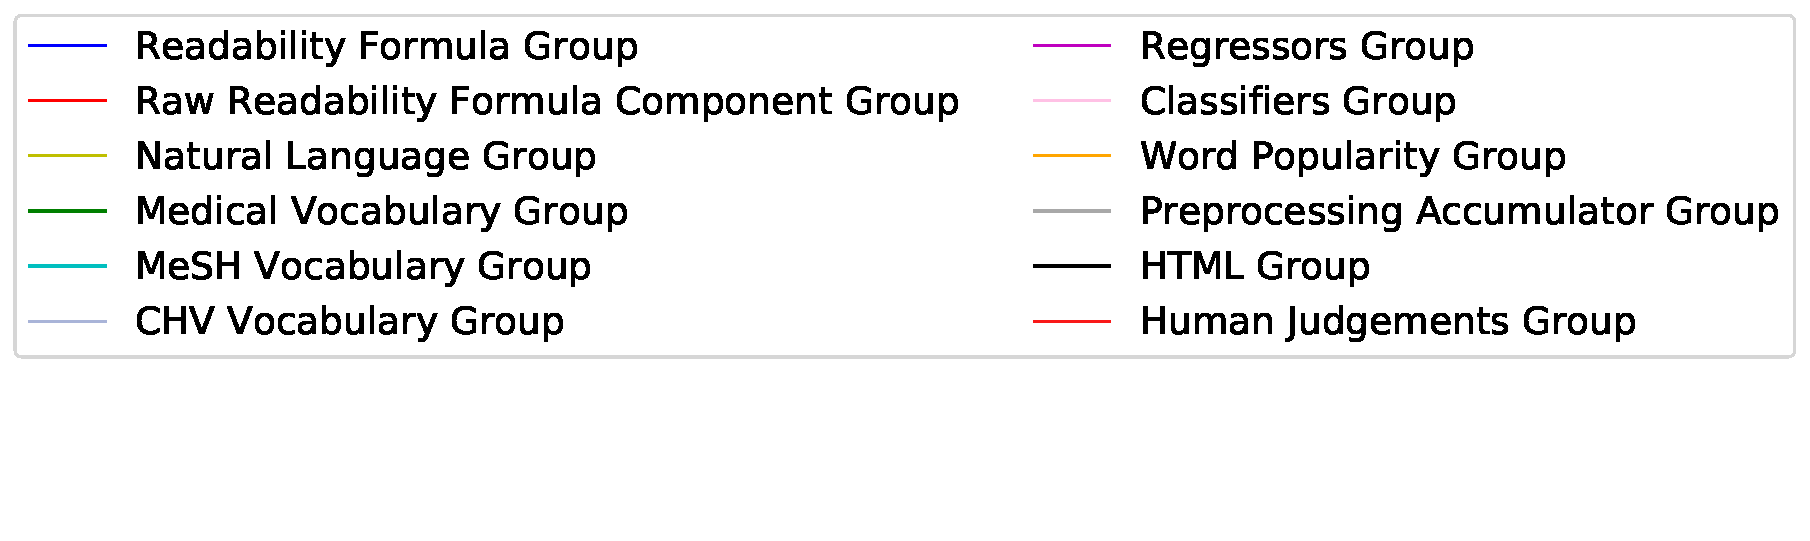
\includegraphics[width=0.65\textwidth]{graphics/legendCorr}
    \vspace{-1.cm}
    \caption{Box plots divided by feature groups. Correlations are calculated using understandability labels from relevant documents assessed in CLEF eHealth 2016}
   \label{fig:boxplot_corr_docs_2016}
\end{figure}

Figure~\ref{fig:boxplot_corr_docs_2015} shows the correlations for CLEF eHealth 2015 assessments.
The choice of preprocessing method had the highest impact on the traditional readability formula group, with the Naive preprocessing clearly underperforming the other preprocessing methods. The choice of the Naive method was also the worst with the raw readability formula components and word frequency estimators, but, interestingly, it was a good choice, if not the best one, for all other groups.
The highest correlations were archived by the regressors and classifiers, independently of the preprocessing method used.

%For this group, all correlation measures point out that the Naive processing yielded the weakest correlation, and Justext was marginally better than Boilerpipe. Comparing the medians, the strategy of DoNotForcePeriod performed better than ForcePeriod. The readability formula group was also the one with higher correlation, with an average correlation equal or higher than the human one.

Similarly to Figure~\ref{fig:boxplot_corr_docs_2015}, Figure~\ref{fig:boxplot_corr_docs_2016} reports the findings for CLEF eHealth 2016. This time, though, the Naive preprocessing method was clearly underperforming for most of the groups analysed, including regressors and classifiers.

In order to further understand our experiments, we compared the median of each pair of preprocessing strategy showed in Figures~\ref{fig:boxplot_corr_docs_2015} and~\ref{fig:boxplot_corr_docs_2016} and present the results in Table~\ref{tab:comparison_preprocessing}. 
For instance, the entry \textit{FP < DNFP} counts the number of times the median value for ForcePeriod was superior to DoNotForcePeriod when comparisons with the same HTML cleaning method was used, e.g. Naive ForcePeriod versus Naive DoNotForcePeriod. From all comparisons, the ones that were statistically significant according to a t-test are shown inside parentheses.

The upper part of Table~\ref{tab:comparison_preprocessing} shows results for the comparisons between ForcePeriod (FP) and DoNotForcePeriod (DNFP). Although the interpretation of readability formulas is drastically affected by this choice of preprocessing, as learning in Chapter~\ref{chp:preprocessing}, the correlation results are not.
The number of times FP reached a higher correlation than DNFP is roughly the same that DNFP was higher than FP.
The bottom part of Table~\ref{tab:comparison_preprocessing} shows the comparisons made for Naive, Justext and Boilerpipe. Results for CLEF 2015 contrast with 2016, while Naive was sightly better than Boilerpipe and Justext in 2015, it was the worst in almost all 2016 comparisons. Also, the comparisons between Justext and Boilerpipe are exactly the opposite from 2015 to 2016.

%
\begin{table}
\centering    
\caption{Exhaustive Comparison summary using the data from Figures 1.2 and 1.3. Numbers inside parentheses represent the number of tests that yielded p < 0.05 in a two-tailed t-test}
\label{tab:comparison_preprocessing}

\resizebox{1.\textwidth}{!}{
\begin{tabular}{lllllllll}
\toprule
\multirow{2}{*}{\textbf{Comparison}} & \multicolumn{4}{c}{\textbf{CLEF 2015}} & \multicolumn{4}{c}{\textbf{CLEF 2016}}\tabularnewline
\cmidrule(l{2pt}r{2pt}){2-5} \cmidrule(l{2pt}r{2pt}){6-9} 
& \textbf{Pearson} & \textbf{Spearman} & \textbf{Kendall Tau} & \textbf{Total} & \textbf{Pearson} & \textbf{Spearman} & \textbf{Kendall Tau} & \textbf{Total}\tabularnewline
\midrule
FP > DNFP & 8 (0) & 11 (4) & 11 (3) & 30 (7) & 16 (10) & 10 (3) & 11 (4) & 37 (17)\tabularnewline
FP < DNFP & 16 (5) & 12 (5) & 12 (6) & 40 (16) & 8 (0) & 12 (2) & 11 (2) & 31 (4)\tabularnewline
FP == DNFP & 0 & 1 & 1 & 2 & 0 & 2 & 2 & 4\tabularnewline
\midrule
Naive > Justext & 11 (7) & 9 (6) & 9 (5) & 29 (18) & 1 (0) & 0 (0) & 0 (0) & 1 (0)\tabularnewline
Naive < Justext & 6 (4) & 8 (4) & 8 (4) & 22 (12) & 16 (12) & 17 (13) & 17 (13) & 50 (38)\tabularnewline
Naive == Justext & 0 & 0 & 0 & 0 & 0 & 0 & 0 & 0\tabularnewline
Naive > Boilerpipe & 12 (7) & 10 (6) & 10 (5) & 32 (18) & 0 (0) & 0 (0) & 0 (0) & 0 (0)\tabularnewline
Naive < Boilerpipe & 5 (4) & 7 (3) & 7 (3) & 19 (10) & 16 (12) & 17 (13) & 17 (13) & 51 (39)\tabularnewline
Naive == Boilerpipe & 0 & 0 & 0 & 0 & 0 & 0 & 0 & 0\tabularnewline
Justext > Boilerpipe & 10 (7) & 16 (9) & 14 (8) & 40 (24) & 9 (4) & 9 (4) & 4 (2) & 17 (8)\tabularnewline
Justext < Boilerpipe & 7 (2) & 1 (0) & 3 (1) & 11 (3) & 8 (2) & 8 (2) & 13 (2) & 34 (6)\tabularnewline
Boilerpipe == Justext & 0 & 0 & 0 & 0 & 0 & 0 & 0 & 0\tabularnewline
\bottomrule 
\end{tabular}
} % close resizebox
\end{table}

%

\section{Experimenting with Understandability}
\label{sec:experiments}

Our experiments are based on the data collected during the Information Retrieval branch of CLEF eHealth. To the best of our knowledge that was the only venue in which topical and understandability assessments were collected. 
We show here experiments with the CLEF eHealth 2016 campaign leaving 2015 experiments offline\footnote{Link to experiments will be available upon acceptance of this manuscript}.

We start by the defining the evaluation measure that we will use here. 
In CLEF eHealth campaign, organizers used a modification of RBP which ties together document relevance any other relevance dimension, in this case in particular, understandability \cite{clef16}.
Mathematically, it consists in adding an understandability factor to the RBP formula: $uRBP(\rho) = (1 - \rho) \sum_{k=1}^{K} \rho^{K-1} r(d@K) u(d@k)$, with r(d@k) representing the gain in retrieving a topically relevant documents at rank $k$ and u(d@k) the gains coming from the understandability factor of a document at rank $k$.

The drawback of such evaluation metric is that we cannot separately evaluate each dimension. We propose, instead, to separately evaluate a ranking list with respect to its topical relevance and its understandability:
\begin{itemize}
        \item $P_r@10$: a document is topically relevant if assessed as somewhat relevant or highly relevant. This metric counts the number of topically relevant documents in the top 10 documents of a ranked list.
        \item $P_u@10$: a document is relevant for this metric if the understandability score is smaller than a threshold $U$. Like $P_r@10$, we count the number of relevant documents in the first 10 documents of a ranked list. We use $U = 40$ in our experiments. \todo{I decided to use this threshold based on the data. I will need to add a figure to support this clam, I think.}
\end{itemize}

During the campaign, organizers opt to use shallow pools and focus on highly ranked documents, using $P_r@10$ as one official metric for topical relevance.
It makes our choice of metric natural. Likewise it is traditionally done with F measure, we combine $P_r@10$ and $P_u@10$ with an harmonic mean: $F_{ru} = 2 \times \frac{P_r@10 \times P_u@10}{P_r@10 + P_u@10}$. 

When reranking runs, we risk to bring to the top of the rankings documents that were not assessed when the task took place. For this reason, we inform the average percentage of documents that were not assessed in the top 10 documents of each run (Unj@10) and we inform $P_r@10*$, $P_u@10*$ and $F_{ru}*$, modified measures that excluding all unassessed documents for the ranking list before evaluation.
These last three metrics showcase the potential of a run if it had been included in the pool set.

We start our experiments by showing at the top of Table~\ref{tab:experiments} (indices 1-4) the performance of the top 3 systems in CLEF eHealth 2016 together with a straightforward BM25 baseline run made with Terrier toolkit. Our further experiments will use not only these runs as a comparison base, but modify these runs when necessary.

The first batch of experiments, indices 5-8, consists of reranking the top 20 documents based solely on the Dale-Chall index, as it was the metrics with highest correlation with human judgements for this collection.
The topical relevance of the reranked resulting lists is immediately hurt in benefit of understandability. Note how $P_r@10$ and $P_r@10*$ decrease while $P_u@10$ and in special $P_u@10*$ increase.
The percentage of unassessed documents reach 10\% and, unfortunately, only looking at RBP and uRBP we cannot see the understandability benefits brought by the rerank method.

The next batch of experiments, indices 9-19, swaps the Dale-Chall Index by a Linear Regression (LR) learned using the top features of Table~\ref{tab:top_corr_metrics}\footnote{Experiments with various machine learning methods were performed as well and will be available in a website upon paper acceptance. The results of other methods are similar}. 
We experiment with reranking the top 15 (more more conservative method), 20 and 50 (a more heterodox method). We clearly see the trade-off between understandability and relevance when we increase from top 15 to top 50: while the $P_r@10$ falls 5 points, $P_u@10$ increases 10. Nevertheless, $F_{ru}*$ shows that more conservative methods provide the best trade-offs.
When comparing the use of Dale-Chall and Linear Regression reranking the same number of documents (indices 13-16), we notice that LR results for $P_u@10*$ are always superior to Dale-Chall, meaning it does a better job when bringing the easier documents to the top of the rank, but that not necessarily means the final rank is better, as we can see comparing the results for $F_{ru}*$.

Our third batch of experiments, indices 20-31, aims to combine the good ranking for topicality coming from the original rank list with the best rankings for understandability, coming from the LR reranking.
For that, we use the Reciprocal Rank Fusion (RRF) method, which combines runs on the rank of documents instead of scores~\cite{cormack09}. Reranking with LR and combining runs with RRF allows to obtain the best trade-offs so far, with $F_{ru}$ of the best method in CLEF being improved from 39.05 to 39.68, with comes from a very small decrease in $P_u@10*$ (from 31.70 to 31.60) and a 4.9\% increase in $P_u@10*$ (from 50.83 to 53.30).

Our final batch of experiments, indices 32-34, are based on learning-to-rank. We decided to use the pairwise implementation of the gradient boosting approach from the XGBoost framework~\cite{chen16} due to its recent good results in many machine learning tasks \todo{actually, I should use XGBoost method instead of LR}. Evaluating other learning to rank methods and frameworks are left as future work.
We evaluated three different settings based on the plain BM25 run shown in index 4, each one with a different combination of feature set and relevance labels:
\begin{itemize}
    \item Index 32: we used as relevance labels only the topical labels and as feature set the score of different information retrieval models (BM25, Dirichlet LM and PL2). This represents the typical use of learning to rank aiming to optimize only the topical relevance results. Unfortunately that was not the case and not even the $P_r@10*$ was improved.
    \item Index 33: we used as relevance labels the linear combination of topical relevance and understandability. Additionally to the IR features, we used the 10 features correspondent to the best features according to Kendall tau in Table~\ref{tab:top_corr_metrics}. Results show that this resulted in higher $F_{ur}*$ when compared to its correspondent approaches (indices 4, 8, 12, 16, 19, 23, 27 and 31) due to a high increase in $P_r@10*$, which reveals understandability features improving topicability.
    \item Index 34: On top of our previous run, we included here all features shown in Table~\ref{tab:doc_features}. Note that despite the very high number of unassessed documents, this run shows improvements even in $P_r@10$ obtaining the same results as the third best run in the campaign (ECNU). In its turn, the $P_{r}*$ which ignores the unassessed documents is 8.4\% higher than the best system, while $F_{ru}*$ is 5.2\% higher.
\end{itemize}


\begin{table*}[ht!]
\caption{Results obtained by integrating understandability estimations within
retrieval methods on CLEF 2016. Baseline runs are reported at table
indices 1-3. Re-ranking experiments are reported at indices 4-21.
Fusion experiments are reported at indices 22-30. Learning to rank
experiments are reported at indices 31-35. All measures were calculated
up to rank $n=10$. }
%\vspace{-0.2cm}
 \label{tab:experiments} 
\resizebox{1.00\textwidth}{!}{ %
\begin{tabular}{cclllllllllllll}
\toprule 
    \multirow{2}{*}{Index }  & \multirow{2}{*}{Rerank }  & \multirow{2}{*}{Run }  & \multicolumn{4}{l}{Official CLEF 2016 Metrics} & \multicolumn{8}{l}{New Metrics to Evaluate Underst. in Retrieval - Sec.~\ref{sec:data}}\tabularnewline
\cmidrule(l{2pt}r{2pt}){4-7} \cmidrule(l{2pt}r{2pt}){8-15}  &  &  & $RBP$  & RBP Res.  & uRBP  & uRBP Res.  & $RBP_{u}$  & $RBP_{u}$ Res. & $HRBP$  & HRBP Res. & Unj  & $RBP_{r}^{*}$  & $RBP_{u}^{*}$  & $HRBP^{*}$\tabularnewline
\midrule 
1  & \multirow{3}{*}{No Rerank}  & GUIR~\cite{soldaini16} (Best Run)  & \textbf{28.11}  & 7.65  & \textbf{18.12}  & 7.19  & \textbf{45.69}  & 8.86 & \textbf{25.61}  & 6.50 & 0.01  & \textbf{28.29}  & \textbf{46.03}  & \textbf{25.79} \tabularnewline
2  &  & ECNU~\cite{song16} (Runner Up)  & 27.70  & 7.37  & 17.55  & \textbf{7.34}  & 43.89$^{\diamond}$  & 8.66 & 25.35  & 6.26 & 0.01  & 27.77  & 44.18$^{\diamond}$  & 25.48 \tabularnewline
3  &  & Plain BM25 Baseline  & 25.28$^{\diamond}$  & \textbf{8.24}  & 16.05$^{\diamond}$  & 6.94  & 42.08$^{\diamond}$  & \textbf{10.97} & 22.97$^{\diamond}$  & \textbf{7.19} & \textbf{0.06}  & {26.01}$^{\diamond}$  & {43.89}$^{\diamond}$  & {23.93}$^{\diamond}$ \tabularnewline
\midrule 
4  & \multirow{3}{*}{\makecell{Dale-Chall Top 15}}  & Based on GUIR  & 24.70$^{\dagger\diamond}$  & 8.70  & 16.83$^{\dagger\diamond}$  & 7.27  & 49.10$^{\dagger\diamond}$  & 10.62 & 24.94  & 7.50 & 0.03  & 25.24$^{\dagger\diamond}$  & 50.33$^{\dagger\diamond}$  & 25.54 \tabularnewline
5  &  & Based on ECNU  & 24.78$^{\dagger\diamond}$  & 7.83  & 16.64$^{\diamond}$  & 7.16  & 48.88$^{\dagger\diamond}$  & 9.71 & 24.80  & 6.50 & 0.02  & 25.12$^{\dagger\diamond}$  & 49.64$^{\dagger\diamond}$  & 25.21 \tabularnewline
6  &  & Based on BM25  & 23.22$^{\dagger\diamond}$  & 8.78  & 15.85 $^{\diamond}$  & 6.94  & 47.09$^{\dagger\diamond}$  & 11.83 & 24.01  & 7.42 & 0.07  & 24.04$^{\dagger\diamond}$  & 48.60$^{\dagger\diamond}$  & 24.82 \tabularnewline
\hdashline 7  & \multirow{3}{*}{\makecell{Dale-Chall Top 20}}  & Based on GUIR  & 22.19$^{\dagger\diamond}$  & 9.37  & 15.36$^{\dagger\diamond}$  & 6.98  & 48.71$^{\dagger\diamond}$  & 12.30 & 23.21$^{\dagger\diamond}$  & 8.12 & 0.06  & 23.26$^{\dagger\diamond}$  & 51.39$^{\dagger\diamond}$  & 24.45$^{\dagger\diamond}$\tabularnewline
8  &  & Based on ECNU  & 23.01$^{\dagger\diamond}$  & 8.93  & 15.70$^{\dagger\diamond}$  & 6.91  & 48.99$^{\dagger\diamond}$  & 11.69 & 23.73$^{\dagger\diamond}$  & 7.80 & 0.05  & 23.84$^{\dagger\diamond}$  & 51.00$^{\dagger\diamond}$  & 24.66\tabularnewline
9  &  & Based on BM25  & 21.58$^{\dagger\diamond}$  & 9.51  & 14.83$^{\dagger\diamond}$  & 7.02  & 46.99$^{\dagger}$  & 13.00 & 22.89$^{\diamond}$  & 8.06 & 0.09  & 22.93$^{\dagger\diamond}$  & 49.55$^{\dagger\diamond}$  & 24.26\tabularnewline
\hdashline 10  & \multirow{3}{*}{\makecell{Dale-Chall Top 50}}  & Based on GUIR  & 16.18$^{\dagger\diamond}$  & 15.24  & 11.56$^{\dagger\diamond}$  & 6.80  & 41.79$^{\dagger\diamond}$  & 24.49 & 18.10$^{\dagger\diamond}$  & 14.42 & 0.22  & 20.90$^{\dagger\diamond}$  & 53.28$^{\dagger\diamond}$  & 23.27$^{\dagger\diamond}$ \tabularnewline
11  &  & Based on ECNU  & 16.88$^{\dagger\diamond}$  & 17.37  & 11.78$^{\dagger\diamond}$  & \textbf{7.30}  & 40.76$^{\dagger\diamond}$  & 23.77 & 18.30$^{\dagger\diamond}$  & \textbf{15.57} & \textbf{0.24}  & 21.34$^{\dagger\diamond}$  & 52.07$^{\dagger\diamond}$  & 23.33$^{\dagger\diamond}$ \tabularnewline
12  &  & Based on BM25  & 15.06$^{\dagger\diamond}$  & 15.35$^{\dagger\diamond}$  & 10.55  & 6.62  & 40.03 $^{\diamond}$  & 23.88 & 16.55$^{\dagger\diamond}$  & 13.83 & \textbf{0.24}  & 19.42$^{\dagger\diamond}$  & 51.69$^{\dagger\diamond}$  & 21.59$^{\dagger\diamond}$ \tabularnewline
\hdashline 13  & \multirow{3}{*}{\makecell{XGB Top 15}}  & Based on GUIR  & \textbf{25.16}$^{\dagger\diamond}$  & 8.09  & \textbf{17.27}$^{\dagger\diamond}$  & 7.12  & \textbf{50.96}$^{\dagger\diamond}$  & 10.11 & \textbf{25.16}  & 6.89 & 0.02  & \textbf{25.61}$^{\dagger\diamond}$  & 52.00$^{\dagger\diamond}$  & \textbf{25.68}\tabularnewline
14  &  & Based on ECNU  & 24.18$^{\dagger\diamond}$  & 7.69  & 16.54 $^{\diamond}$  & 7.09  & 50.00$^{\dagger\diamond}$  & 9.91 & 24.56  & 6.65 & 0.02  & 24.56$^{\dagger\diamond}$  & 50.74$^{\dagger\diamond}$  & 25.01\tabularnewline
15  &  & Based on BM25  & 22.33$^{\dagger\diamond}$  & 8.14  & 15.46  & 6.76  & 47.90$^{\dagger\diamond}$  & 12.13 & 22.89$^{\diamond}$  & 7.25 & 0.07  & 23.11$^{\dagger\diamond}$  & 49.43$^{\dagger\diamond}$  & 23.69$^{\diamond}$\tabularnewline
\hdashline 16  & \multirow{3}{*}{\makecell{XGB Top 20}}  & Based on GUIR  & 22.38$^{\dagger\diamond}$  & 9.49  & 15.61$^{\dagger\diamond}$  & 7.05  & 50.45$^{\dagger\diamond}$  & 12.08 & 23.30$^{\dagger\diamond}$  & 8.16 & 0.05  & 23.62$^{\dagger\diamond}$  & 52.98$^{\dagger\diamond}$  & 24.68\tabularnewline
17  &  & Based on ECNU  & 22.95$^{\dagger\diamond}$  & 8.82  & 15.95$^{\dagger\diamond}$  & 7.02  & 50.42$^{\dagger\diamond}$  & 11.70 & 23.97$^{\diamond}$  & 7.56 & 0.04  & 23.68$^{\dagger\diamond}$  & 52.15$^{\dagger\diamond}$  & 24.73\tabularnewline
18  &  & Based on BM25  & 20.65$^{\dagger\diamond}$  & 9.42  & 14.46$^{\dagger\diamond}$  & 6.84  & 47.74$^{\dagger\diamond}$  & 13.56 & 21.93$^{\diamond}$  & 8.34 & 0.09  & 21.98$^{\dagger\diamond}$  & 50.28$^{\dagger\diamond}$  & 23.27$^{\diamond}$\tabularnewline
\hdashline 19  & \multirow{3}{*}{\makecell{XGB Top 50}}  & Based on GUIR  & 16.65$^{\dagger\diamond}$  & 15.73  & 12.39$^{\dagger\diamond}$  & 6.84  & 43.49$^{\dagger\diamond}$  & 23.63 & 18.70$^{\dagger\diamond}$  & 13.74 & 0.22  & 21.13$^{\dagger\diamond}$  & \textbf{55.07}$^{\dagger\diamond}$  & 23.58$^{\dagger\diamond}$\tabularnewline
20  &  & Based on ECNU  & 16.19$^{\dagger\diamond}$  & \textbf{17.01}  & 11.82$^{\dagger\diamond}$  & 7.27  & 43.05$^{\diamond}$  & \textbf{24.75} & 18.27$^{\dagger\diamond}$  & 14.41 & \textbf{0.24}  & 20.16$^{\dagger\diamond}$  & 54.70$^{\dagger\diamond}$  & 22.96$^{\dagger\diamond}$\tabularnewline
21  &  & Based on BM25  & 15.43$^{\dagger\diamond}$  & 15.37  & 11.33$^{\dagger\diamond}$  & 6.48  & 41.93$^{\diamond}$  & 23.65 & 17.43$^{\dagger\diamond}$  & 13.40 & 0.26  & 19.58$^{\dagger\diamond}$  & 54.04$^{\dagger\diamond}$  & 22.17$^{\dagger\diamond}$\tabularnewline
\midrule 
22  & \multirow{3}{*}{\makecell{RRF (XGB \& Orig.) Top 15} }  & Based on GUIR  & \textbf{27.23}$^{\dagger\diamond}$  & 7.76  & \textbf{18.31}  & \textbf{7.23}  & 49.69$^{\dagger\diamond}$  & 9.18 & 26.49$^{\dagger\diamond}$  & 6.62 & 0.01  & \textbf{27.46}$^{\dagger\diamond}$  & 50.07$^{\dagger\diamond}$  & \textbf{26.69}$^{\dagger\diamond}$\tabularnewline
23  &  & Based on ECNU  & 26.60$^{\dagger\diamond}$  & 7.41  & 17.81  & 7.19  & 48.67$^{\dagger\diamond}$  & 8.80 & 26.02  & 6.09 & 0.01  & 26.76$^{\dagger\diamond}$  & 49.10$^{\dagger\diamond}$  & 26.27$^{\dagger}$ \tabularnewline
24  &  & Based on BM25  & 24.57$^{\diamond}$  & 8.15  & 16.51$^{\diamond}$  & 6.91  & 46.76$^{\dagger}$  & 11.23 & 24.16$^{\dagger}$  & 7.20 & 0.06  & 25.32$^{\diamond}$  & 48.52$^{\dagger\diamond}$  & 25.08$^{\dagger}$ \tabularnewline
\hdashline 25  & \multirow{3}{*}{\makecell{RRF (XGB \& Orig.) Top 20}}  & Based on GUIR  & 26.21$^{\dagger\diamond}$  & 7.96  & 17.73  & 7.19  & 50.29$^{\dagger\diamond}$  & 9.58 & 25.89  & 6.73 & 0.03  & 26.53$^{\dagger\diamond}$  & 50.98$^{\dagger\diamond}$  & 26.25\tabularnewline
26  &  & Based on ECNU  & 26.15$^{\dagger\diamond}$  & 7.64  & 17.69  & 7.09  & 49.70$^{\dagger\diamond}$  & 9.28 & \textbf{26.07 } & 6.39 & 0.02  & 26.38$^{\dagger\diamond}$  & 50.32$^{\dagger\diamond}$  & 26.35\tabularnewline
27  &  & Based on BM25  & 24.04$^{\dagger\diamond}$  & 8.24  & 16.32$^{\diamond}$  & 6.87  & 47.69$^{\dagger\diamond}$  & 11.40 & 24.08$^{\dagger\diamond}$  & 7.35 & 0.06  & 24.82$^{\dagger\diamond}$  & 49.52$^{\dagger\diamond}$  & 25.01$^{\dagger}$ \tabularnewline
\hdashline 28  & \multirow{3}{*}{\makecell{RRF (XGB \& Orig.) Top 50}}  & Based on GUIR  & 24.09$^{\dagger\diamond}$  & \textbf{9.44}  & 16.85$^{\dagger\diamond}$  & 7.02  & 50.55$^{\dagger\diamond}$  & 11.76 & 24.76  & \textbf{8.01} & 0.07  & 25.08$^{\dagger\diamond}$  & \textbf{52.84}$^{\dagger\diamond}$  & 25.84\tabularnewline
29  &  & Based on ECNU  & 24.17$^{\dagger\diamond}$  & 8.67  & 16.75$^{\diamond}$  & 7.12  & \textbf{50.63}$^{\dagger\diamond}$  & 11.66 & 25.00  & 7.61 & 0.07  & 24.90$^{\dagger\diamond}$  & 52.50$^{\dagger\diamond}$  & 25.84 \tabularnewline
30  &  & Based on BM25  & 22.28$^{\dagger\diamond}$  & 8.87 & 15.50  & 6.76  & 48.79$^{\dagger\diamond}$  & \textbf{12.90} & 23.13$^{\dagger\diamond}$  & 7.82 & \textbf{0.10 } & 23.46$^{\dagger\diamond}$  & 51.89$^{\dagger\diamond}$  & 24.57\tabularnewline
\midrule 
31  & \multirow{5}{*}{XGB LeToR}  & Combo 1 on BM25  & 20.42$^{\dagger\diamond}$  & 17.61  & 13.00$^{\dagger\diamond}$  & 7.41  & 32.17$^{\dagger\diamond}$  & 24.61 & 18.39$^{\dagger\diamond}$  & 14.41 & 0.28  & 25.25$^{\diamond}$  & 43.19$^{\diamond}$  & 23.83$^{\diamond}$\tabularnewline
32  &  & Combo 2 on BM25  & 24.98$^{\dagger\diamond}$  & 19.83  & 15.30$^{\dagger\diamond}$  & 8.09  & 35.09$^{\dagger\diamond}$  & 25.14 & 22.26$^{\diamond}$  & 17.50 & 0.24  & 30.41  & 46.09  & 28.28$^{\dagger\diamond}$ \tabularnewline
33  &  & Combo 3 on BM25  & 26.35$^{\dagger}$  & \textbf{20.48}  & 15.88$^{\dagger\diamond}$  & 8.16  & 34.73$^{\dagger\diamond}$  & 24.69 & 21.81$^{\dagger}$  & 17.41 & 0.22  & 32.25$^{\diamond}$  & 45.44  & 28.22$^{\dagger\diamond}$\tabularnewline
34  &  & Combo 4 on BM25  & 16.16$^{\dagger\diamond}$  & 19.48  & 10.76$^{\dagger\diamond}$  & 7.27  & \textbf{36.75}$^{\dagger\diamond}$  & \textbf{28.51} & 16.77$^{\dagger\diamond}$  & \textbf{17.80} & \textbf{0.29 } & 22.20$^{\dagger\diamond}$  & \textbf{50.06}$^{\dagger\diamond}$  & 23.32$^{\diamond}$\tabularnewline
35  &  & Combo 5 on BM25  & \textbf{26.76}$^{\diamond}$  & \textbf{20.48}  & \textbf{16.19}$^{\diamond}$  & \textbf{8.34}  & 35.26$^{\dagger\diamond}$  & 24.13 & \textbf{22.96}  & 17.59 & 0.22  & \textbf{32.60}$^{\dagger}$  & 45.87  & \textbf{29.20}$^{\dagger\diamond}$\tabularnewline
\bottomrule
\end{tabular}
} % end of resizebox
\end{table*}





\section{Conclusion}
\label{sec:conclusion_doc_analysis}

There is an abundance of factors that affect how readability is perceived by users. 
In this chapter we devised and studied a large number of readability estimators, ranging from traditional readability formulas extensively used in the past 50 years to state-of-the-art machine learning algorithms.
We grouped them into semantically related groups in order to visualize their correlation with human assessments collected during CLEF eHealth campaigns in 2015 and 2016.

Complementary to our previous chapter, we evaluated how preprocessing steps impact the readability estimation in traditional readability formulas and in other modern estimators. We empirically learnt the importance of preprocessing steps when applying readability formulas, as the highest correlations happen when other than the Naive method is used.
For the most modern estimators, such as the ones based on machine learning methods, the correlation is less sensible to the preprocessing steps.

We also studied the correlation of each individual readability formula to the human assessment to provide insights on which formula should be preferred. Our analysis concluded that the Simple Measure of Gobbledygook (SMOG) and Dale-Chall Index (DCI) were the most correlated metrics for the two datasets studied and, together with Coleman-Liau Index (CLI) and the Flesch Reading Ease (FRE) are the most stable metrics across datasets, and therefore, should be preferred.

Finally, this chapter serves as a basis for the following chapters of this work, as the learning to rank methods will largely use the estimators devised and analysed here.

%MISSING - POSSIBLE TODOs:
% * I will use the evaluations from CLEF eHealth 2015 and 2016 to conclude that for the same topic, we can find very different results in respect to their understandability (readability) score. I might want to hire some people to classify how hard a topic is. Then I could correlate that with the mean scores of documents for that topic.
% * I will try to come up with some sort of reasoning behind the understandability judgements: is it because of the text length? number of hard (long or out of dictionary) words?

%\mytodo{In this chapter I could add other readability measures later, such as the neural network ones (see cikm 2017)}

